\documentclass[10pt,twoside,a4paper]{article}

% Configure these parameters.
% Name and email
\newcommand{\studentname}{Zijun Joe Yan}
\newcommand{\studentemail}{zy275@cam.ac.uk}

% Date work done
\newcommand{\svworkdate}{2016-11-13}

% Details of supervision
\newcommand{\svcourse}{CST Part IA: Digital Design}
\newcommand{\svnumber}{1}
\newcommand{\svdate}{2016-11-15}
\newcommand{\svtime}{18:30}
\newcommand{\svvenue}{Churchill Seminar Room 1}
\newcommand{\svrname}{Dr Matthew Ireland}
\newcommand{\svrinit}{JKF}
% End configuration

\usepackage{a4}             % Adjust margins for A4 media
\usepackage{fancyhdr}
\renewcommand{\headrulewidth}{0.4pt}
\renewcommand{\footrulewidth}{0.4pt}
\fancyheadoffset[LO,LE,RO,RE]{0pt}
\fancyfootoffset[LO,LE,RO,RE]{0pt}
\pagestyle{fancy}
\fancyhead{}
\fancyhead[LO,RE]{{\bfseries \studentname}\\\studentemail}
\fancyhead[RO,LE]{{\bfseries \svcourse, SV~\svnumber}\\\svdate\ \svtime, \svvenue}
\fancyfoot{}
\fancyfoot[LO,RE]{For: \svrname}
\fancyfoot[RO,LE]{\thepage\ / \pageref{LastPage}}
\fancyfoot[C]{\today}

\usepackage{lastpage}       % "n of m" page numbering
\usepackage{lscape}         % Makes landscape easier
%\usepackage{portland}      % Switch between portrait and landscape
\usepackage{graphics}       % Graphics commands
\usepackage{wrapfig}        % Wrapping text around figures
\usepackage{epsfig}         % Embed encapsulated postscript
\usepackage{rotating}       % Extra graphics rotation
%\usepackage{tables}        % Tabular environments
\usepackage{longtable}      % Page breaks within tables
\usepackage{supertabular}   % Page breaks within tables
\usepackage{multicol}       % Allows table cells to span cols
\usepackage{multirow}       % Allows table cells to span rows
\usepackage{texnames}       % Macros for common tex names
%\usepackage{trees}         % Tree-like layout
\usepackage{hhline}         % Horizontal lines in tables
\usepackage{siunitx}        % Correct spacing of units

\usepackage{listings}       % Source code listings
\usepackage{array}          % Array environment
\usepackage{hyperref}       % URL formatting
\usepackage{amsmath}        % American Mathematical Society
\usepackage{amssymb}        % Maths symbols
\usepackage{amsthm}         % Theorems
%\usepackage{mathpartir}    % Proofs and inference rules
\usepackage{verbatim}       % Verbatim blocks
\usepackage{ifthen}         % Conditional processing in tex
\usepackage{xcolor}         % X11 colour names

% control width and vertically align text in table cells
\newcolumntype{L}[1]{>{\raggedright\let\newline\\\arraybackslash\hspace{0pt}}m{#1}}
\newcolumntype{C}[1]{>{\centering\let\newline\\\arraybackslash\hspace{0pt}}m{#1}}
\newcolumntype{R}[1]{>{\raggedleft\let\newline\\\arraybackslash\hspace{0pt}}m{#1}}

% make hyperref links not-ugly
\hypersetup{
    colorlinks=false,
    pdfborder={0 0 0},
}

\renewcommand{\oddsidemargin}{-20pt}
\renewcommand{\evensidemargin}{-20pt}
\renewcommand{\topmargin}{-30pt}
\renewcommand{\textwidth}{410pt}
\renewcommand{\marginparwidth}{100pt}

\setlength{\parindent}{0em}
\addtolength{\parskip}{1ex}

\usepackage[draft]{changes}
\setauthormarkup[left]{\textbf{[#1]}~}
\definechangesauthor[\svrname]{\svrinit}{orange}
\newcommand{\jkfadd}[1]{\added[\svrinit]{#1}}
\newcommand{\jkfdel}[1]{\deleted[\svrinit]{#1}}
\newcommand{\jkfrep}[2]{\replaced[\svrinit]{#1}{#2}}
\newcommand{\jkfmar}[1]{\marginpar{\jkfadd{#1}}}

\begin{document}

\author{\studentname}
\title{\svcourse, SV~\svnumber}
\date{\svworkdate}

\textbf{\svcourse, SV~\svnumber}\\
\textbf{\studentname}\\
\textbf{\svworkdate}\\

%%%%%%%%%%%%%%%%%%%%%
% Set configuration settings at top of file.
%
% Type out your supervision work, replacing the demo text below.
% The demo text demonstrates how supervisors will mark it by adding, deleting, replacing text, and by commenting in the margin.
% If you arrange your answers into paragraphs sensibly, it'll be easier to understand the supervisor's/supervisors' comments.

% Demo text.  This kid was trying to explain what a compiler was.  He's not a very good student.

\section{Ex1}
\begin{enumerate}
\item[1.1.1]
\begin{tabular}{ccccccc}
$A$ & $B$ & $\bar{a}$ & $\overline{\bar{a}+b}$ & $\bar{b}$ & $\overline{a+\bar{b}}$ & $x$\\
\hline
0&0&1&1&1&1&0\\
0&1&1&0&0&1&1\\
1&0&0&1&1&0&1\\
1&1&0&1&0&1&0\\
\hline
0&0&1&0&1&0&1\\
0&1&1&0&0&1&0\\
1&0&0&1&1&0&0\\
1&1&0&0&0&0&1\\
\end{tabular}\newline\
The first circuit is called XOR.\newline
the second circuit is called NOR.\newline
\item[1.2.1] $a.b.c+a.c.\overline{c}=a.b.(c+\bar{c})=ab$ \newline

\item[1.2.2] $a(\bar{a}+b)=a\bar{a}+ab=0+ab=ab$ \newline
\item[1.2.3] $(a+c)(\overline{a}+b)$ \newline
	  $\overline{a}c+ab+cb$	\newline
	  $\overline{a}c+ab+(\overline{a}+a)cb$\newline 
	  $\overline{a}c+ab$ (adsorbtion) btw. this is consensus \newline
\item[1.2.4] $(a+c)(a+d)(b+c)(b+d)$ \newline
	  $\overline{\overline{a}\overline{c}+\overline{a}\overline{d}+\overline{b}\overline{c}+\overline{b}\overline{d}}$ \newline
	  $\overline{\overline{a}+\overline{b}}+\overline{\overline{c}+\overline{d}}$\newline
	  $ab+cd$
\item[1.2.x]
$x+(\bar{x}y)=(x+\bar{x})(x+y)=1.(x+y)=x+y$\newline
To prove the second equation,take complement on both side.
$\overline{x+(\bar{x}y)}=\overline{x+y}$\newline
Then the LHS will be:$\bar{x}(x+\bar{y}=\bar{x}x+\bar{x}\bar{y}=\bar{x}\bar{y})$\newline

So proved:$\overline{x+y}=\bar{x}\bar{y}$\newline
To prove the third one, just replace x and y with $\bar{x}$ and $\bar{y}$ \newline
and take implement on the both side on the second equation.\newline
so proved:$\bar{x}+\bar{y}=\overline{xy}$
\item[1.7.a]
$a\bar{b}+ac=\overline{\overline{a\bar{b}}.\overline{ac}}$

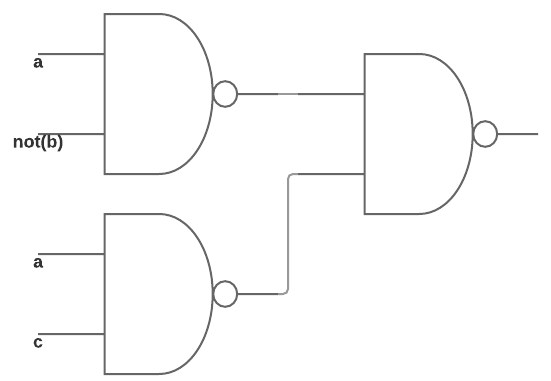
\includegraphics[scale=0.5]{1-7-a.png} 
\item[1.7.b]
$a(\bar{b}+c)=\overline{\overline{\bar{b}+c}+\bar{a}}$

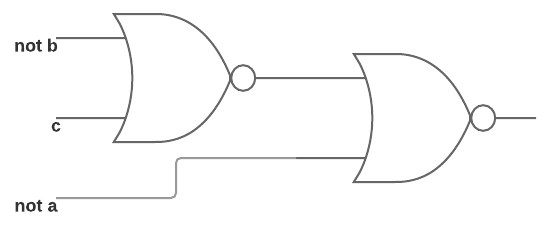
\includegraphics[scale=0.5]{1-7-b.png} 

\item[1.8]
$g=0101+0110+0111+1000$

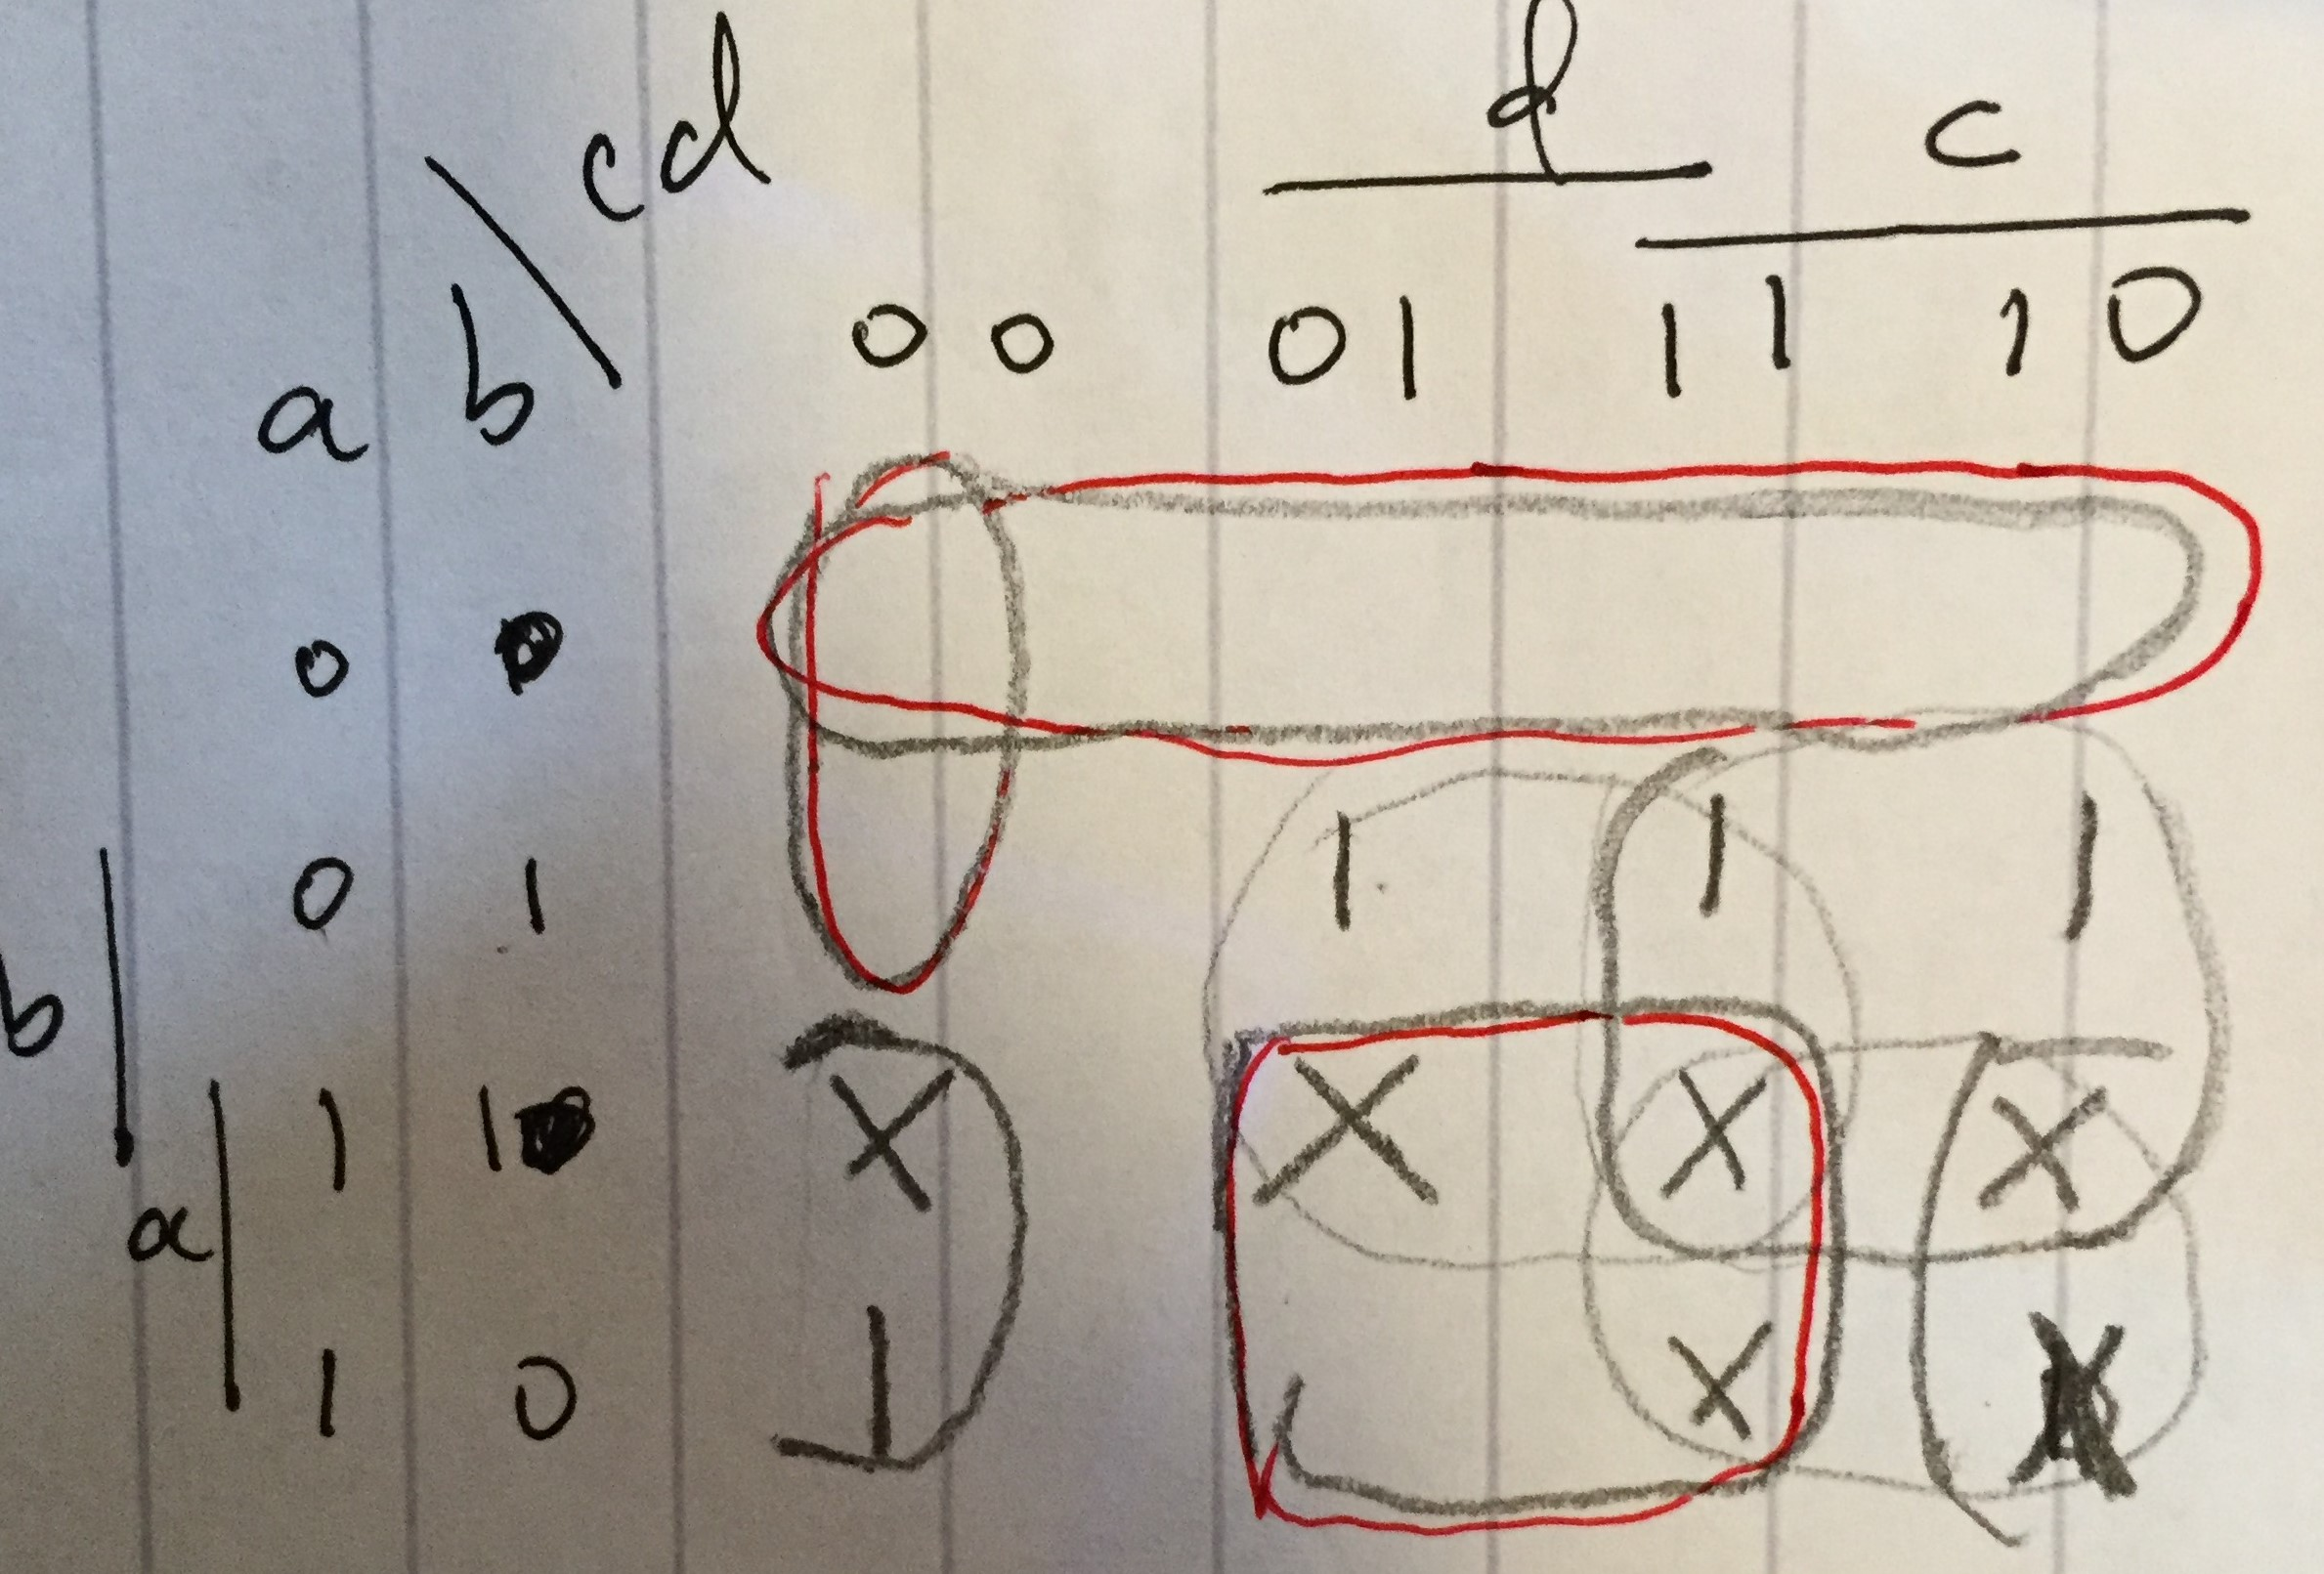
\includegraphics[scale=0.1]{1-8.JPG}\newline
$g=bd+bc+a\bar{d}$\newline
$\bar{g}=\bar{a}\bar{b}+\bar{a}\bar{c}\bar{d}+ad$\newline
$g=(a+b)(a+c+d)(\bar{a}+\bar{d})$

\item[1.11]
(a)100 50 25 12 6 3 1 \newline
   reverse 0010011 is 01100100\newline
   38 19 9 4 2 1 \newline
   reverse 011001 is 100110\newline
   not 00100110 is 11011001\newline
   then +1 is 11011010\newline
   so 100 = 01100100$|_2$ and -38 = 11011010$|_2$   \newline
   01100100 + 11011010= 100111110\newline
   remove head 1 and this is 00111110 or (58)$_{10}$ or (3E)$_{16}$ which is the attempted answer.\newline
   0010 0110 0111 0101 0100 1100 1101 1111 1110 1010\newline
   actually they will go through a properly drawn 4-4 K-map in a zigzag way.
   

\end{enumerate}
\section{Ex2}
I guess those are lists of binary code but no idea how to decode.. 
\section{Ex3}
\begin{enumerate}
\item[(a)] 
There are 16 possibility.\newline
\begin{tabular}{ccc}
$A$ & $B$ & $output$\\
\hline
0   & 0   & x\\
0   & 1   & x\\
1   & 0   & x\\
1   & 1   & x\\
\end{tabular}\newline
One truth table means one possible function.Then to fill each x with 
0 or 1.\newline There are $2^4$ possibility.
\item[(b)]
$\bar{a}=\overline{0+a}$\newline
notice $\overline{\bar{a}+\bar{b}}=a.b$\newline
so $ab=\overline{\overline{0+a}+\overline{0+b}} $
\item[(c)]
$\bar{a}=(0\equiv a)=(1\oplus a)$\newline
$a+b=(ab)\oplus (a\oplus b)$

\end{enumerate}

\section{Ex4}

(a)$\overline{abc...}=\overline{a}+\overline{b}+\overline{c}...\newline
\overline{a+b+c...}=\overline{a}\overline{b}\overline{c}...
$\newline
(b)Minterms:the junction of all variables in complemented or uncomplemented form\newline
   Essential terms: covers a term that no other term covers it. (Do you mean Essential Prime terms or not?)\newline
   prime terms: cannot be further combined.\newline
(c)sum of products form: disjunctions of junction (OR of AND variables).\newline
   minimised sum of products form: simplified SOP by K-map or  Q-M method\newline
   disjunctive normal form: the disjunction of its minterms\newline
(d)All circles are essential prime term.\newline
   minimum SOP:$bd+bc+\bar{a}d+\bar{a}c+a\bar{b}\bar{c}\bar{d}$\newline
   
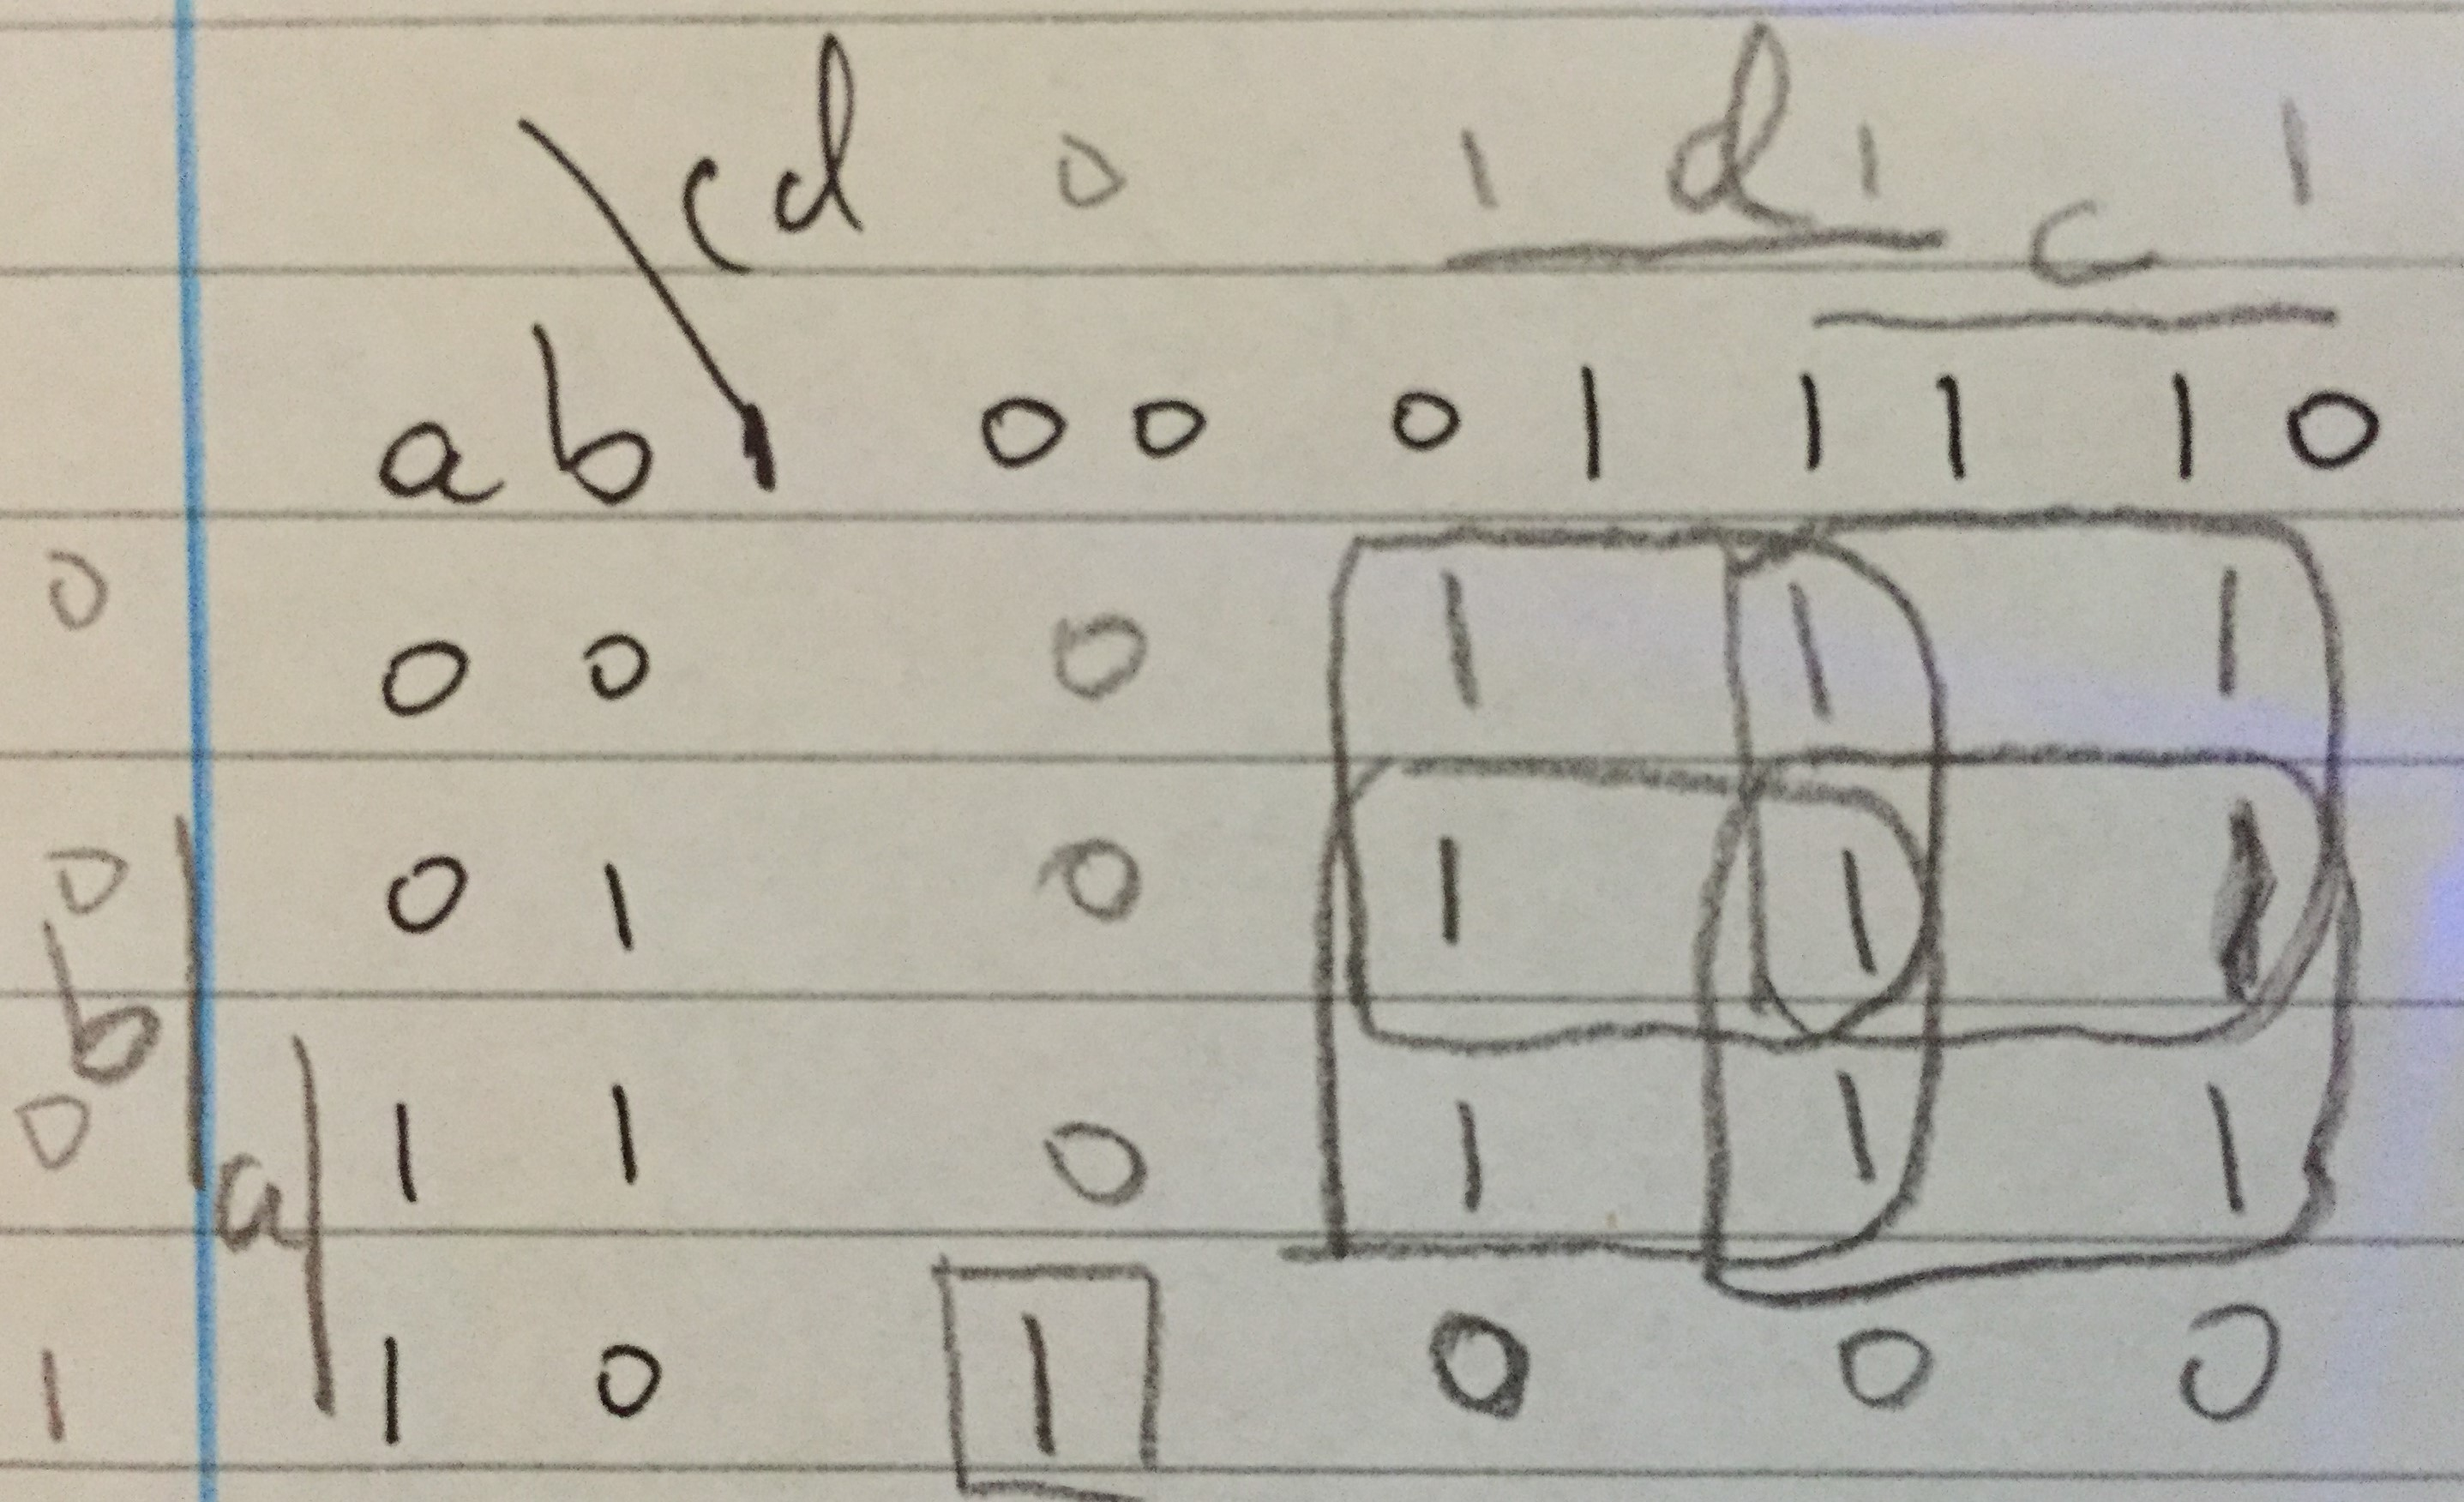
\includegraphics[scale=0.1]{4-d.JPG}

(e)$\bar{a}d+\bar{a}c+a\bar{c}\bar{d}$\newline
(f)$\bar{f}=\bar{a}\bar{c}\bar{d}+b\bar{c}\bar{d}+a\bar{b}d+a\bar{c}d$\newline
minimum POS:$f=(a+c+d)(\bar{b}+c+d)(\bar{a}+b+\bar{d})(\bar{a}+c+\bar{d})$
\section{Ex5}

(a)$(X+Y)(X+Z)\newline
\overline{\bar{X}\bar{Y}+\bar{X}\bar{Z}} \newline
\overline{\overline{X}(\overline{Z}+\overline{Y})} \newline
X+YZ$\newline
(b)The same as 1.2.3 \newline
(c)Tristate Buffer \newline
(d)$(A+B+\bar{C}DE)(A+\bar{D}+E)(\bar{A}+C)\newline
	(AC+\bar{A}(B+\bar{C}DE))(A+\bar{D}+E)\newline
	(AC+\bar{A}B+\bar{A}\bar{C}DE)(A+\bar{D}+E)\newline
	AC+AC\bar{D}+ACE+0+\bar{A}\bar{D}B+\bar{A}BE+0+0+\bar{A}\bar{C}DE\newline
	AC+\bar{A}\bar{D}B+\bar{A}BE+\bar{A}\bar{C}DE$\newline
(e)cell adjacency:010 011 001 000 100 101 111 110 \newline
   method: a(n-1) and reversed a(n-1) then add 0 or 1 to head.\newline
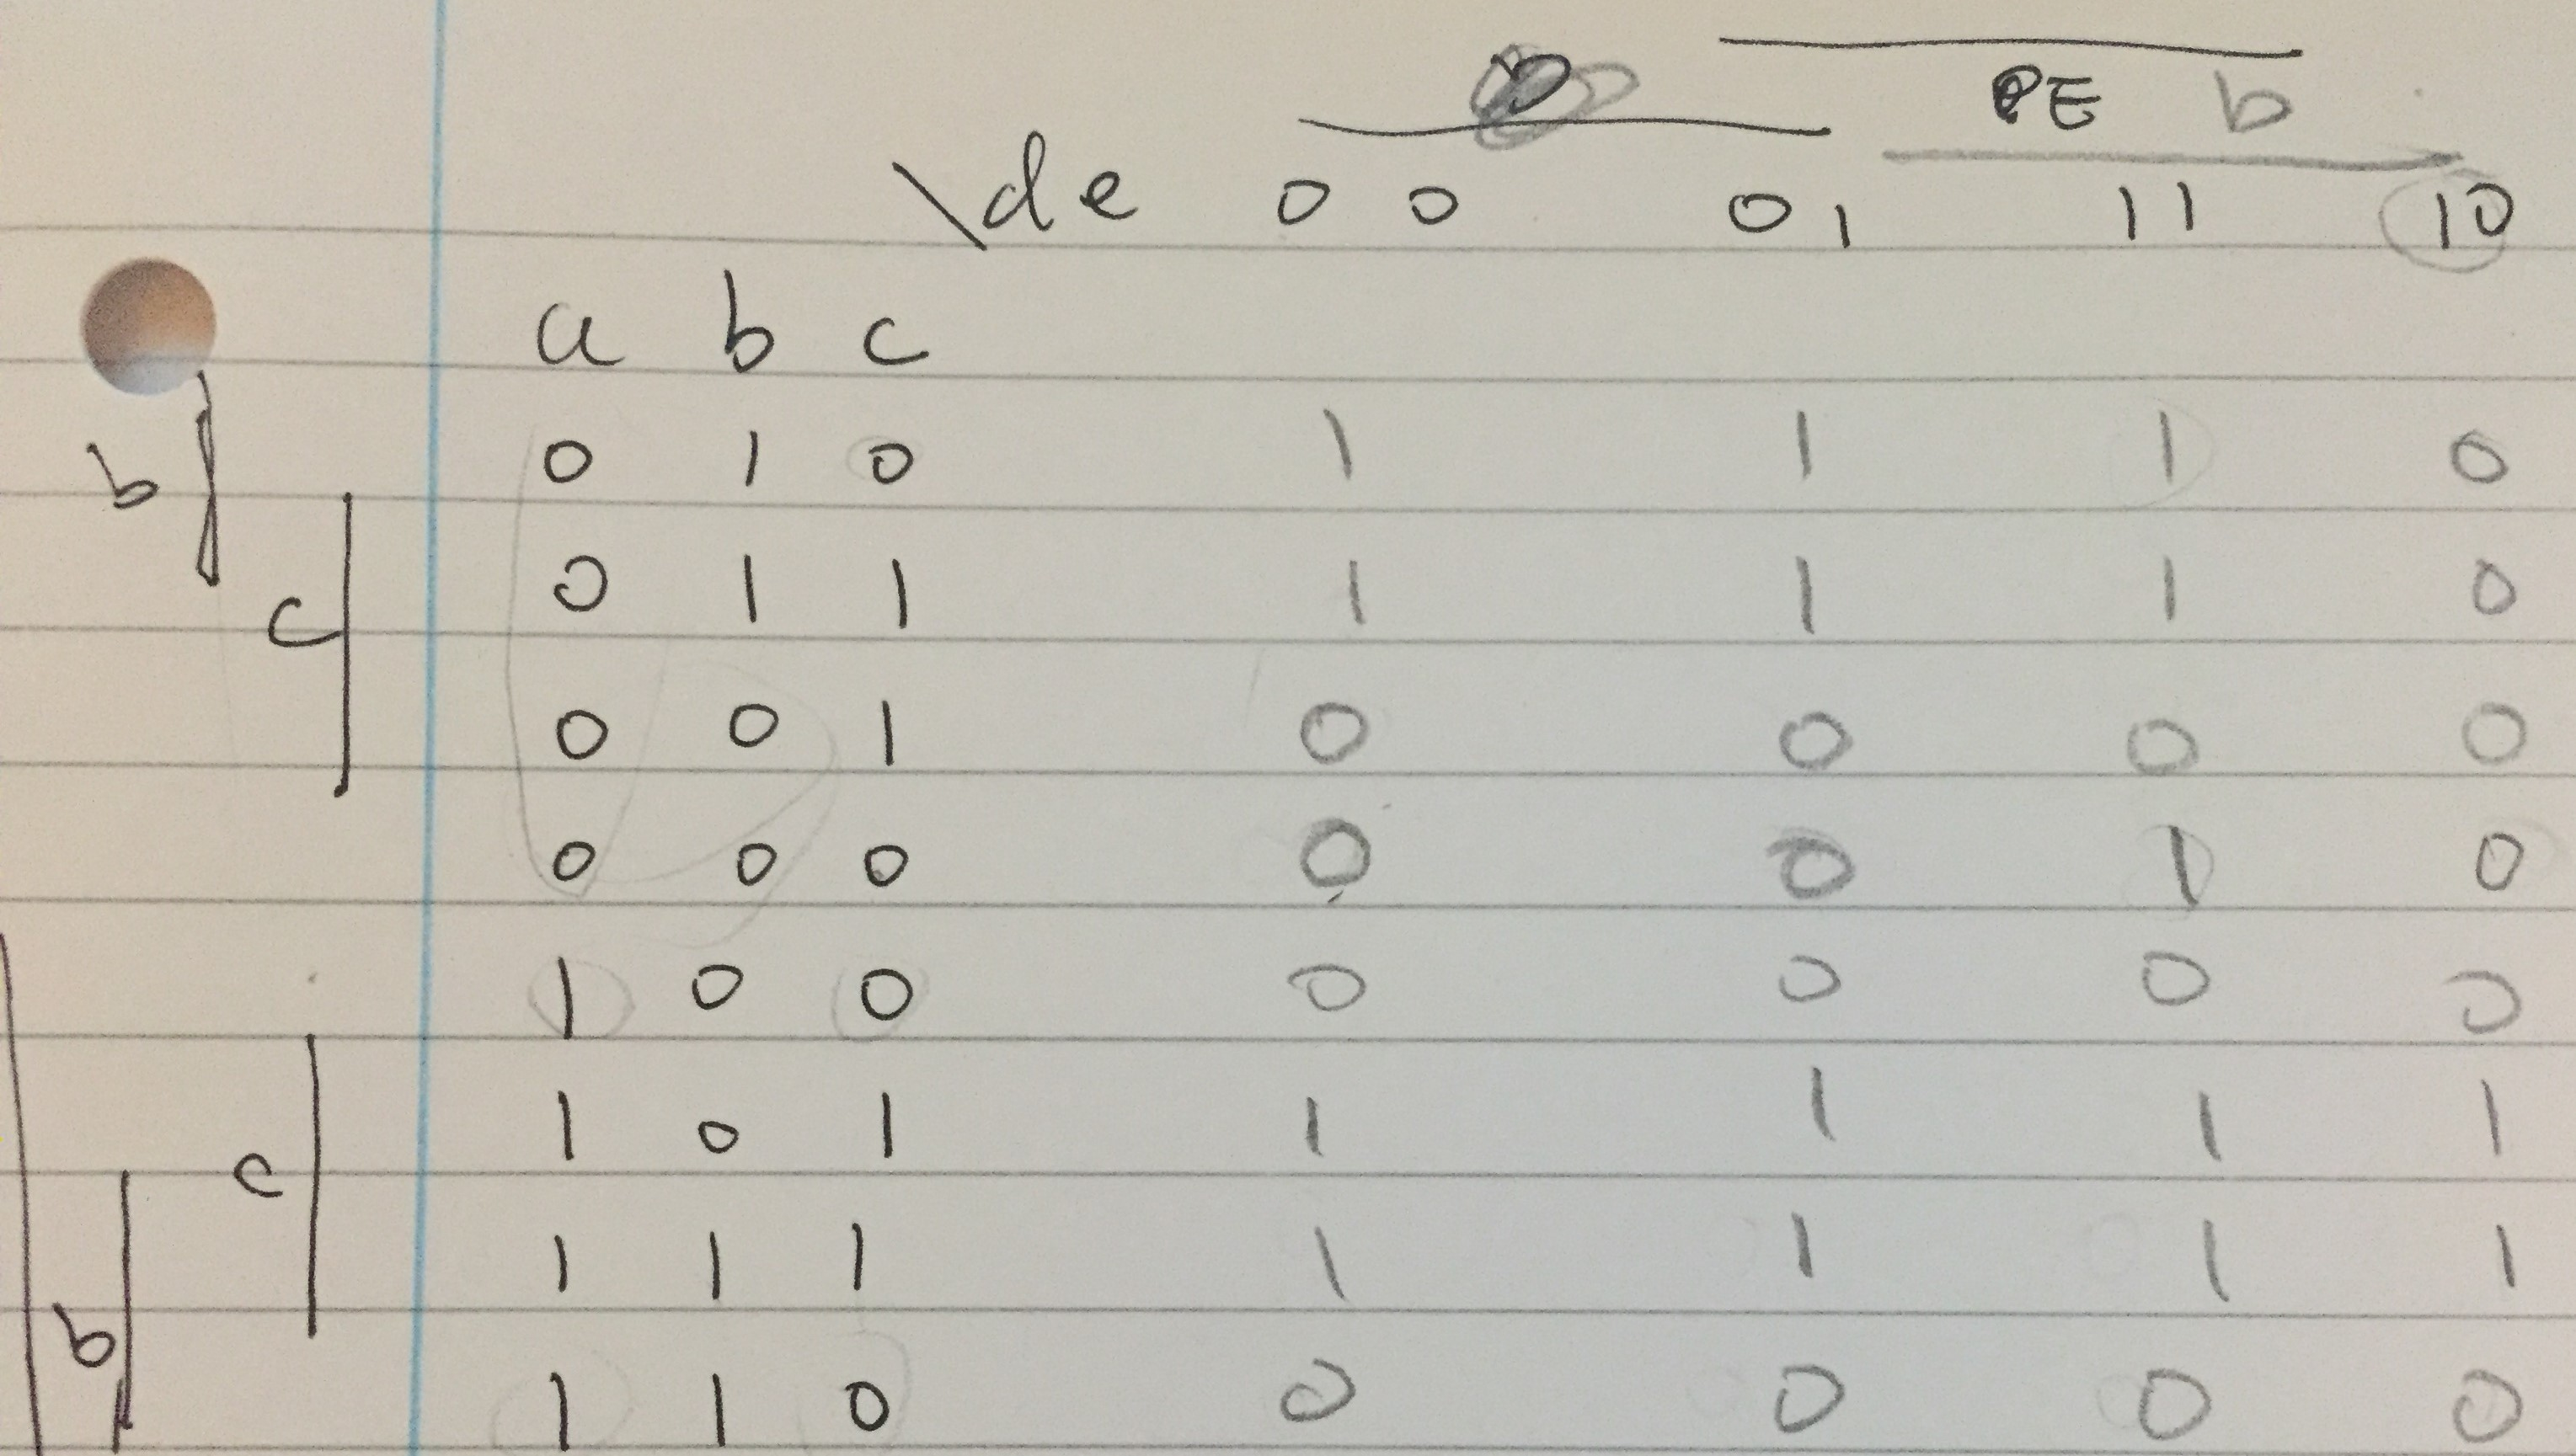
\includegraphics[scale=0.1]{5-e.JPG}\newline
(f)\newline
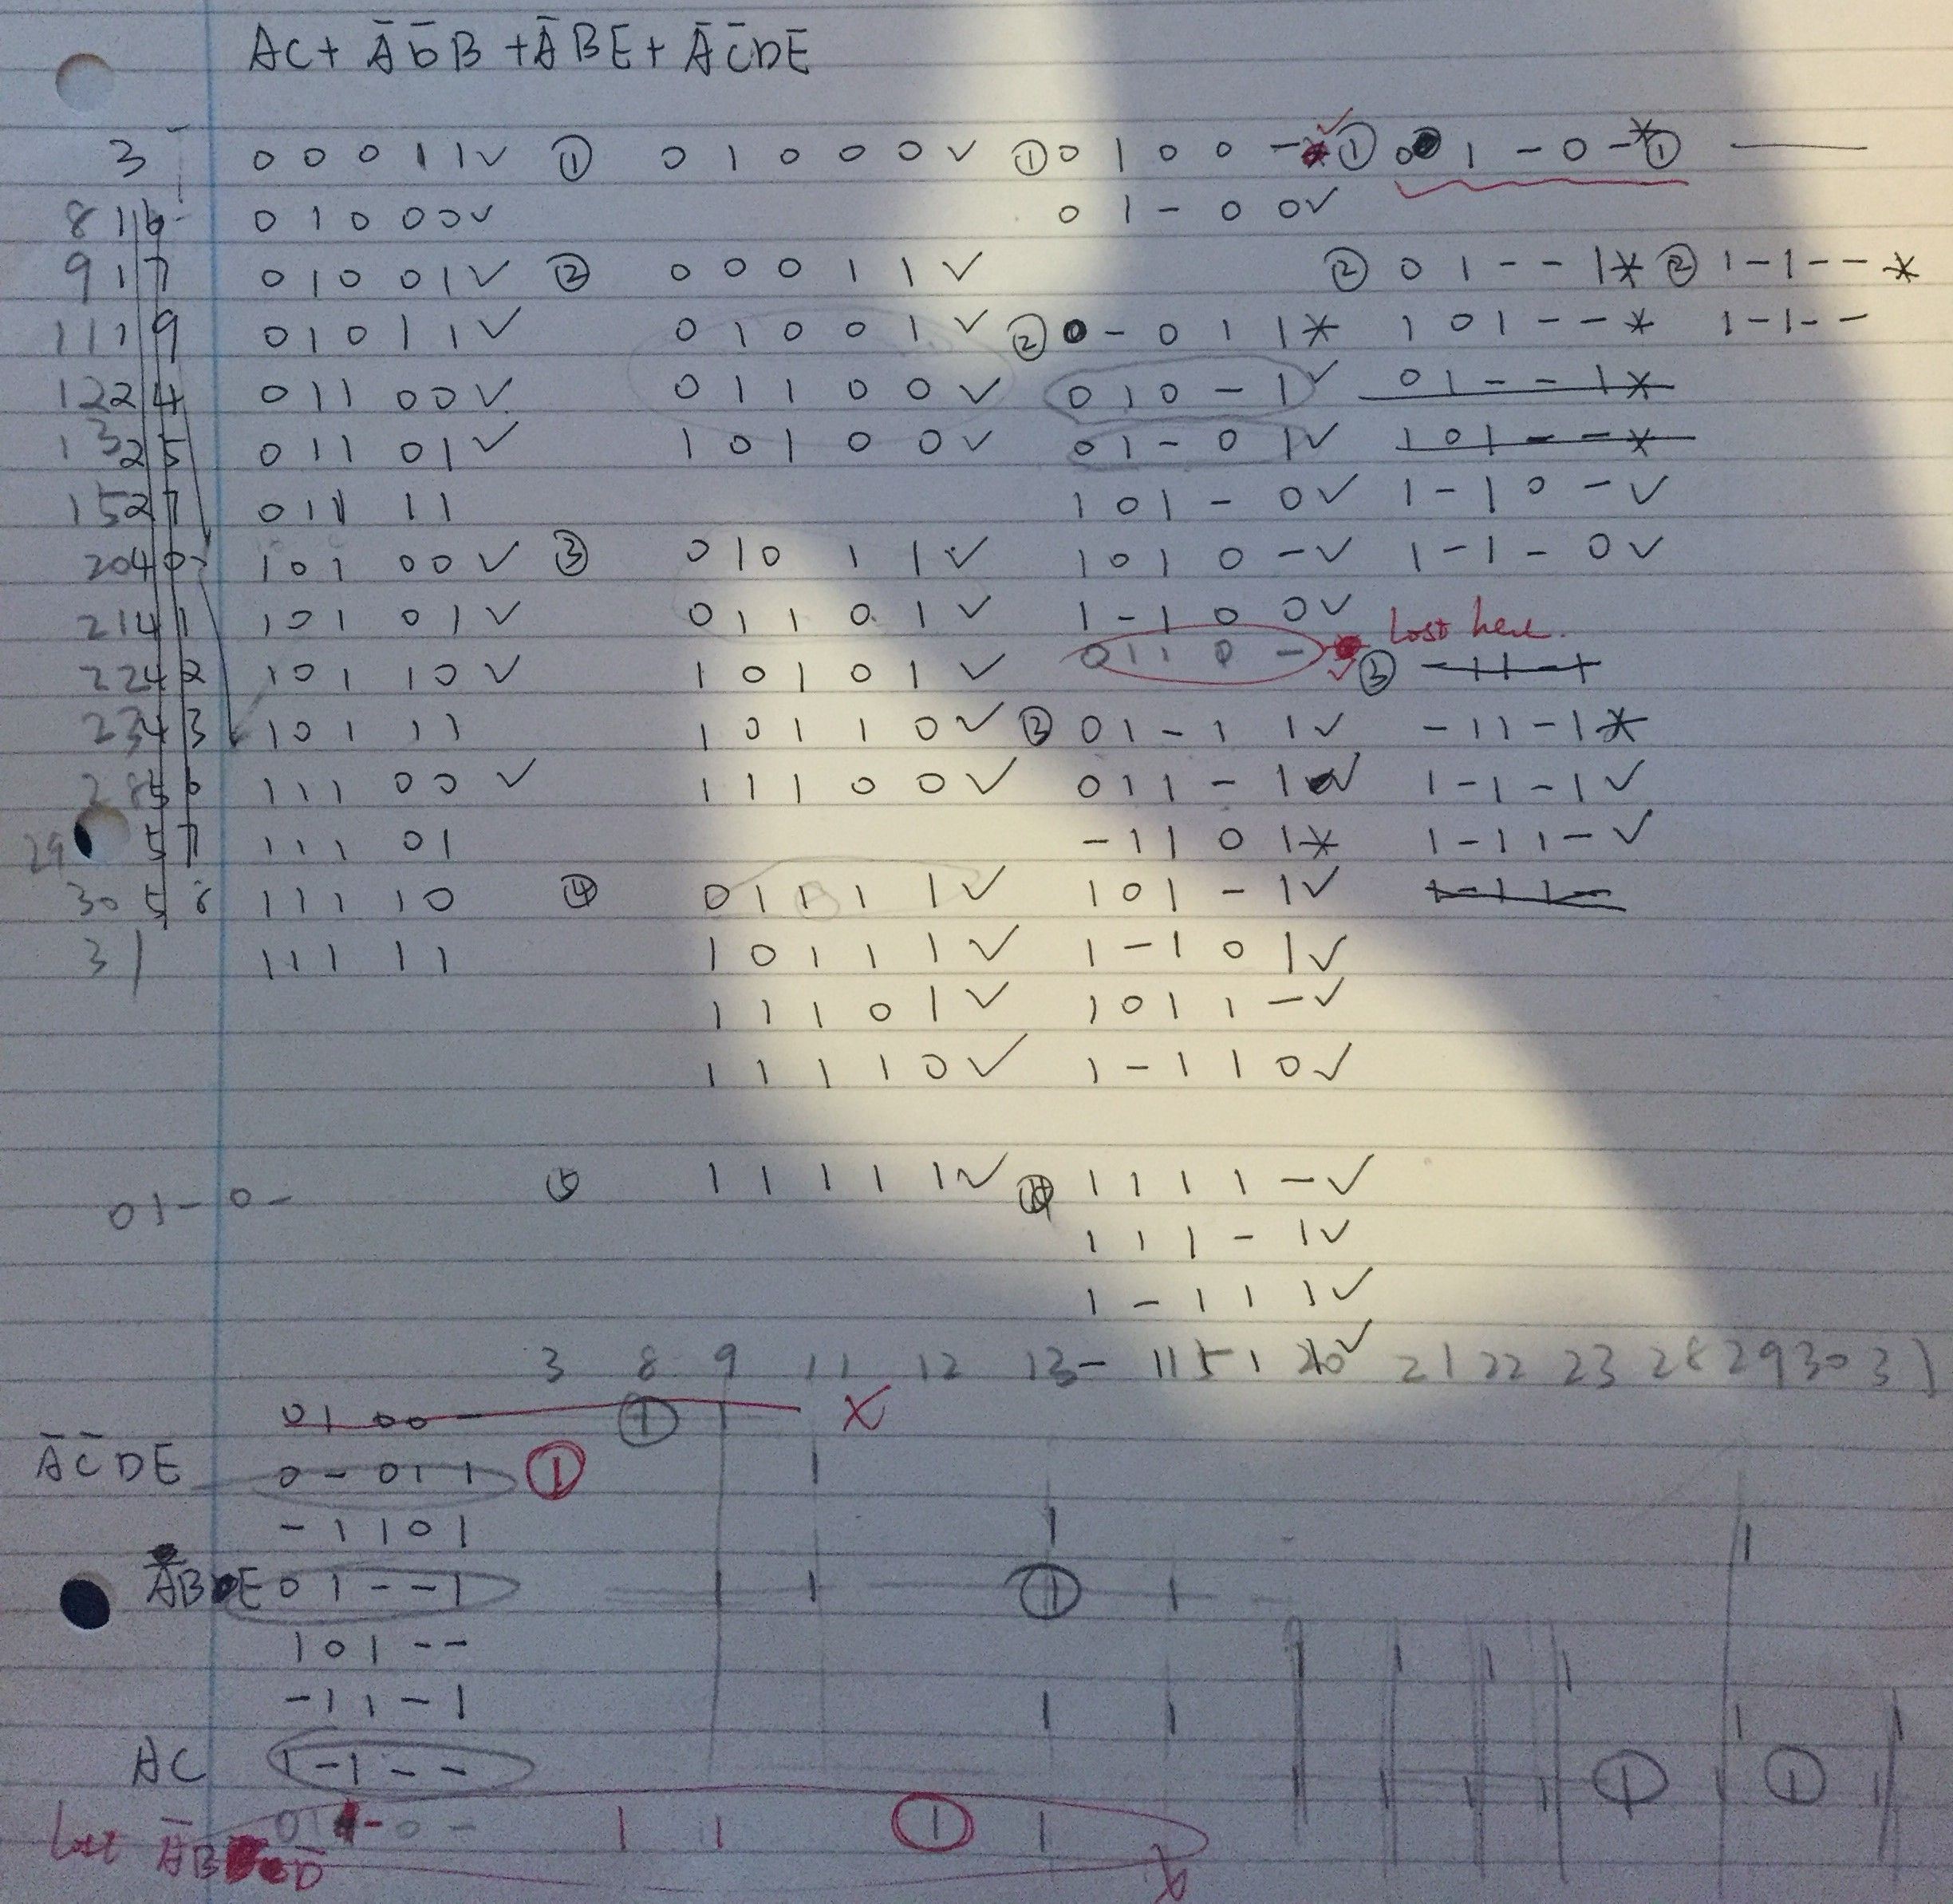
\includegraphics[scale=0.15]{5-f.JPG}


\section{Ex6}

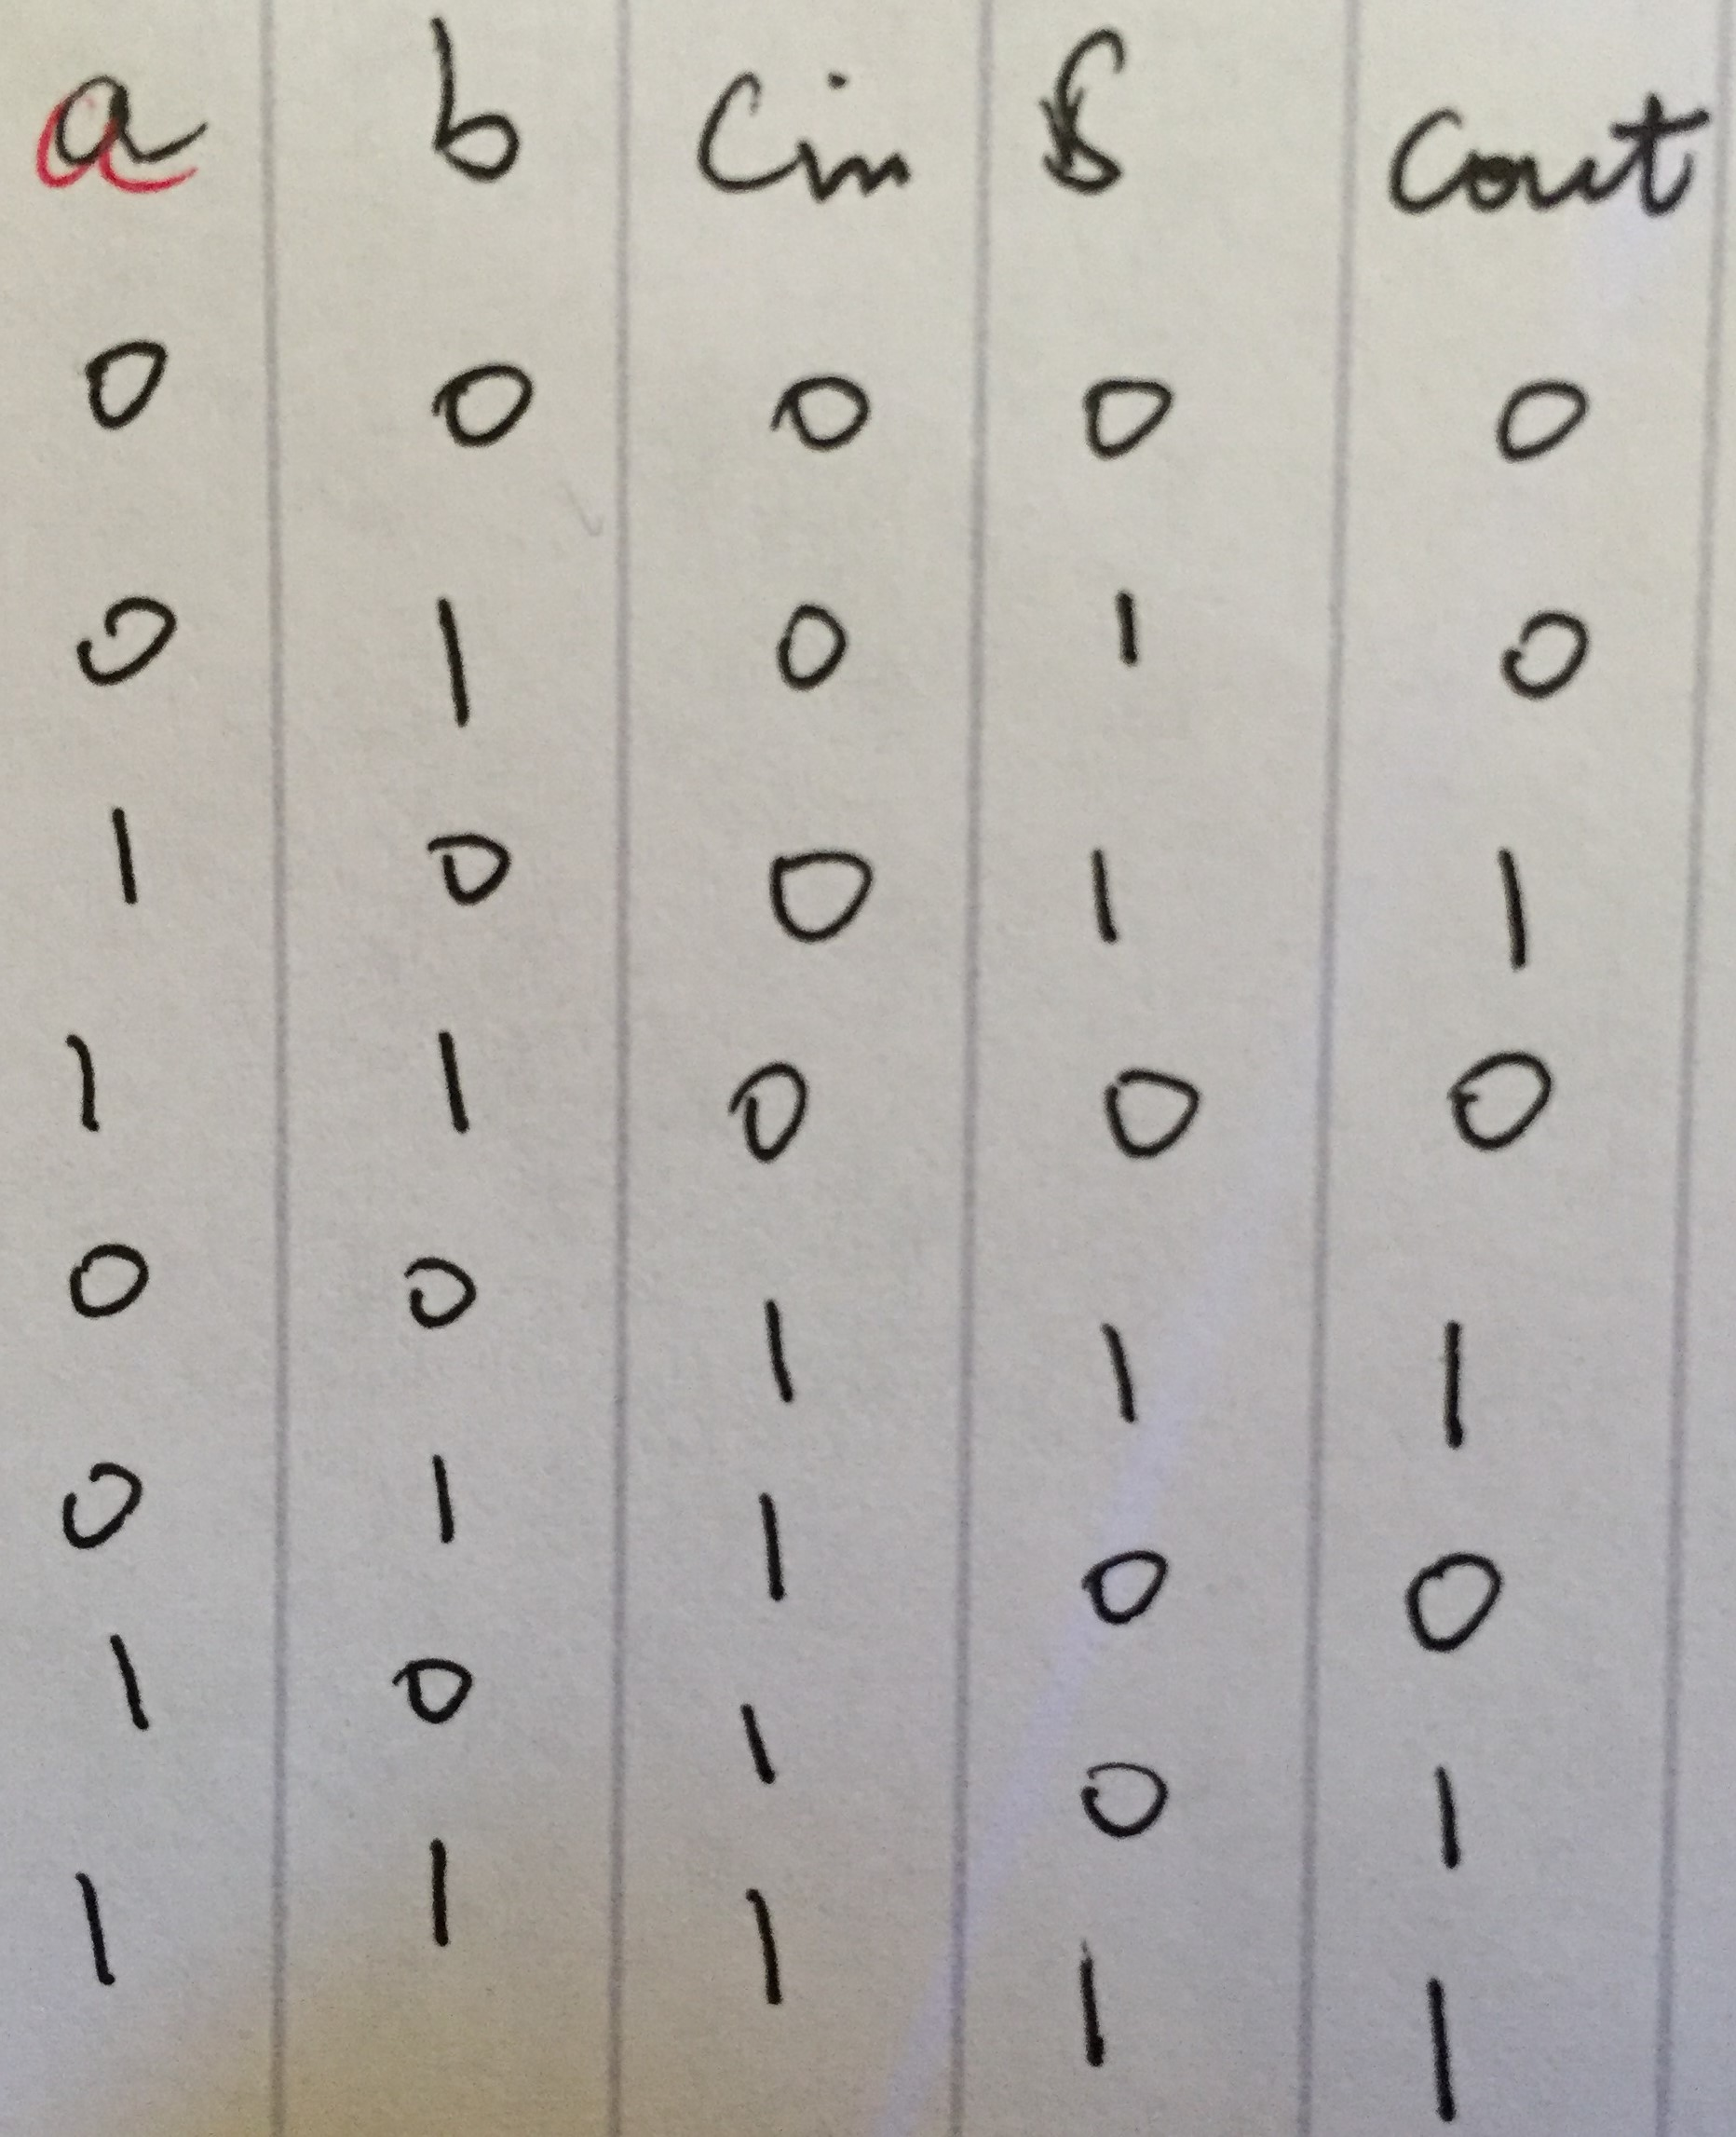
\includegraphics[scale=0.1]{6.JPG} \newline
$s=a\oplus b\oplus c_{in}$\newline
$c_{out}=a.\bar{b}\oplus c_{in}$\newline
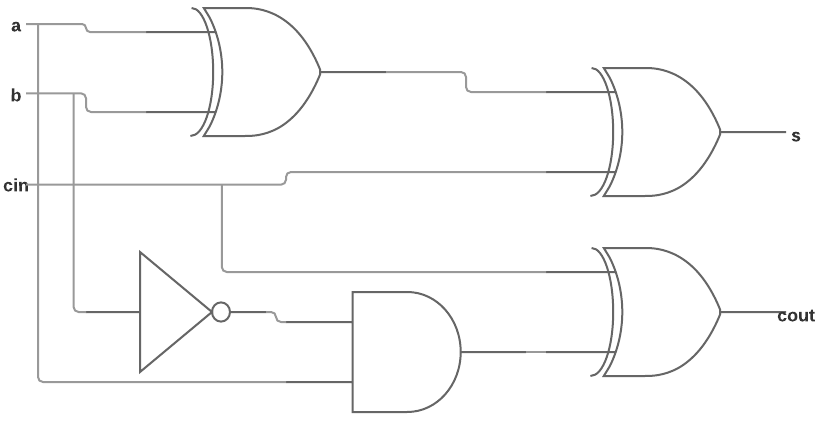
\includegraphics[scale=1]{6(1).png} \newline
\begin{verbatim}
The circuit above have input a b cin and output s and cout.
cin: 1 means need to subtract 1 0 means not.
cout: 1 means need to borrow 1 from higher digital 0 means not.
\end{verbatim}
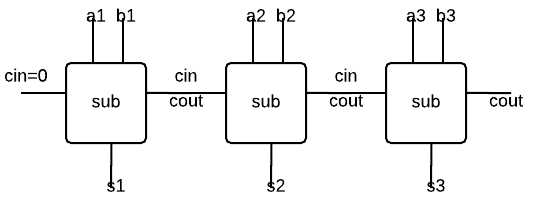
\includegraphics[scale=1]{6(2).png} 



\section{Ex7}
\begin{enumerate}
\item[(a)]

\includegraphics[scale=1]{7.png} 
\item[(b)]
\begin{verbatim}
The 0 0 means clear so once the first input is 0 0 then the output H should also be clear.
For C, once b is logical 0 then it must be 0 (no need for add 1 to next digit) 
otherwise it is also clear 0 0.
\end{verbatim}
\begin{verbatim}
A1 A0 B1 B0 H1 H0 C1 C0 
0 0 0 0 0 0 0 0 
0 0 0 1 0 0 0 1 
0 0 1 0 0 0 0 0 
0 1 0 0 0 0 0 1 
0 1 0 1 0 1 0 1 
0 1 1 0 1 0 0 1 
1 0 0 0 0 0 0 0 
1 0 0 1 1 0 0 1 
1 0 1 0 0 1 1 0
\end{verbatim}
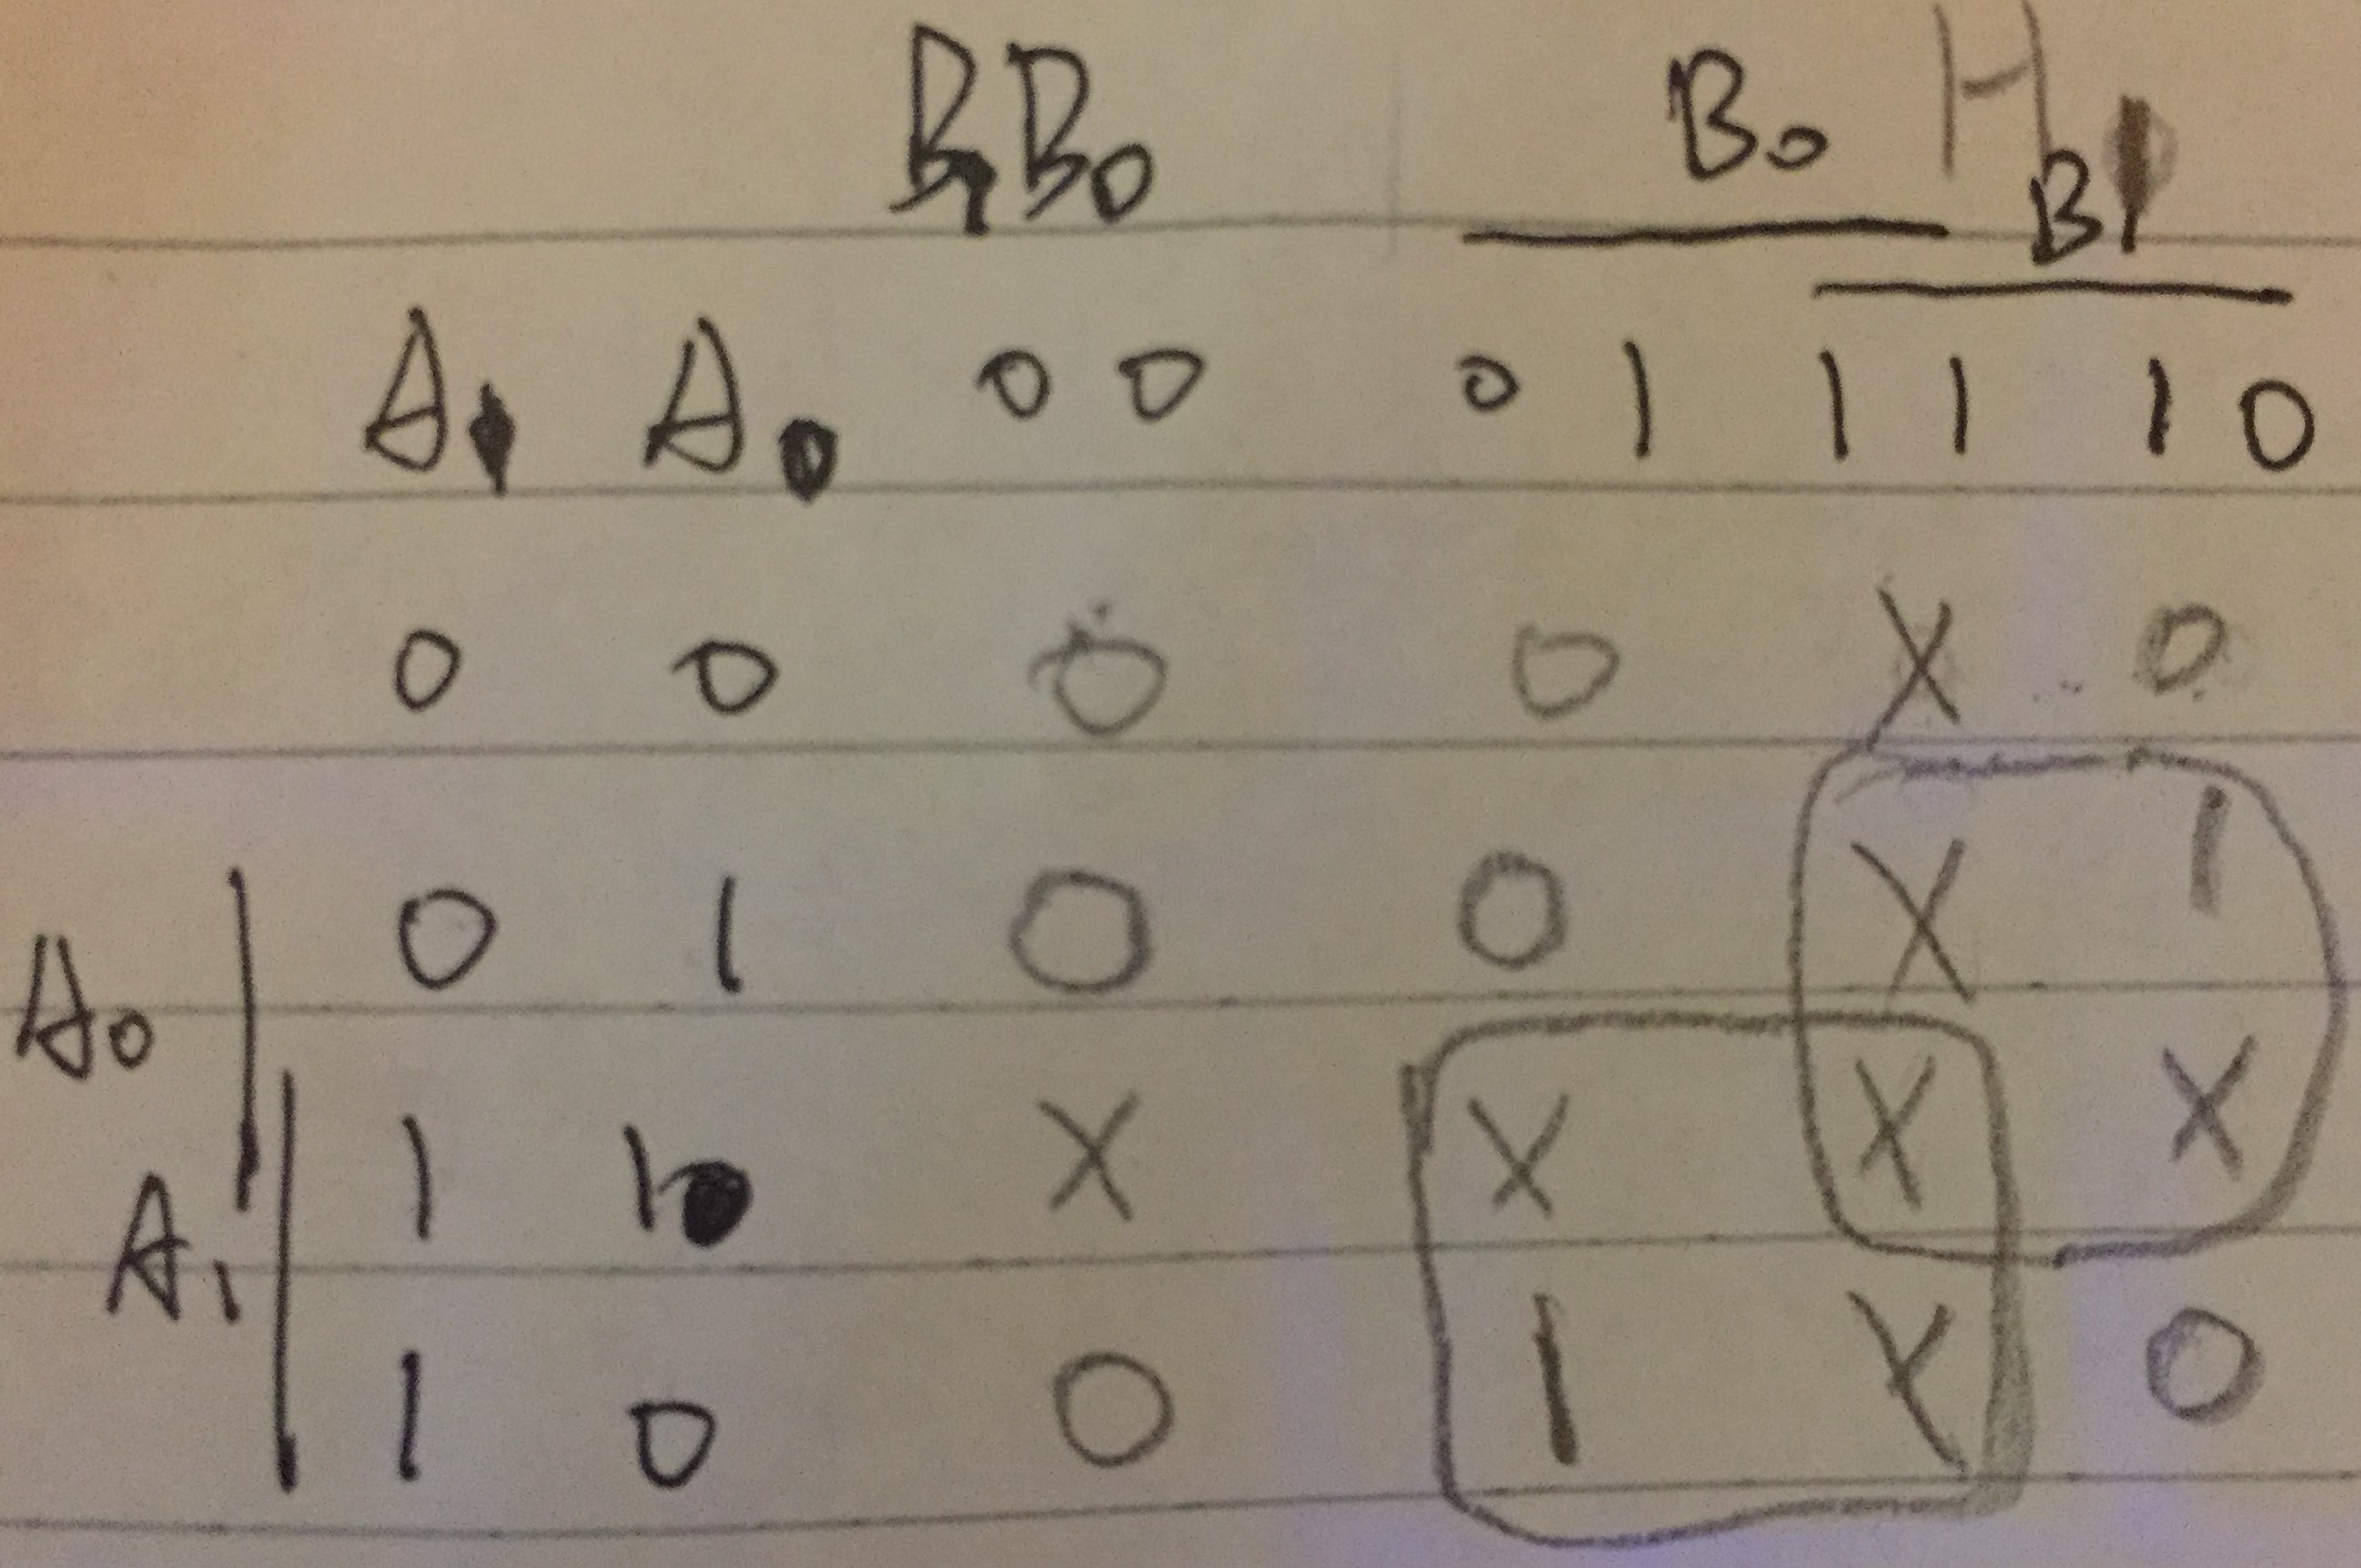
\includegraphics[scale=0.1]{7H1.JPG} 
$H_1 =A_1 B_0 + A_0 B_1$\newline
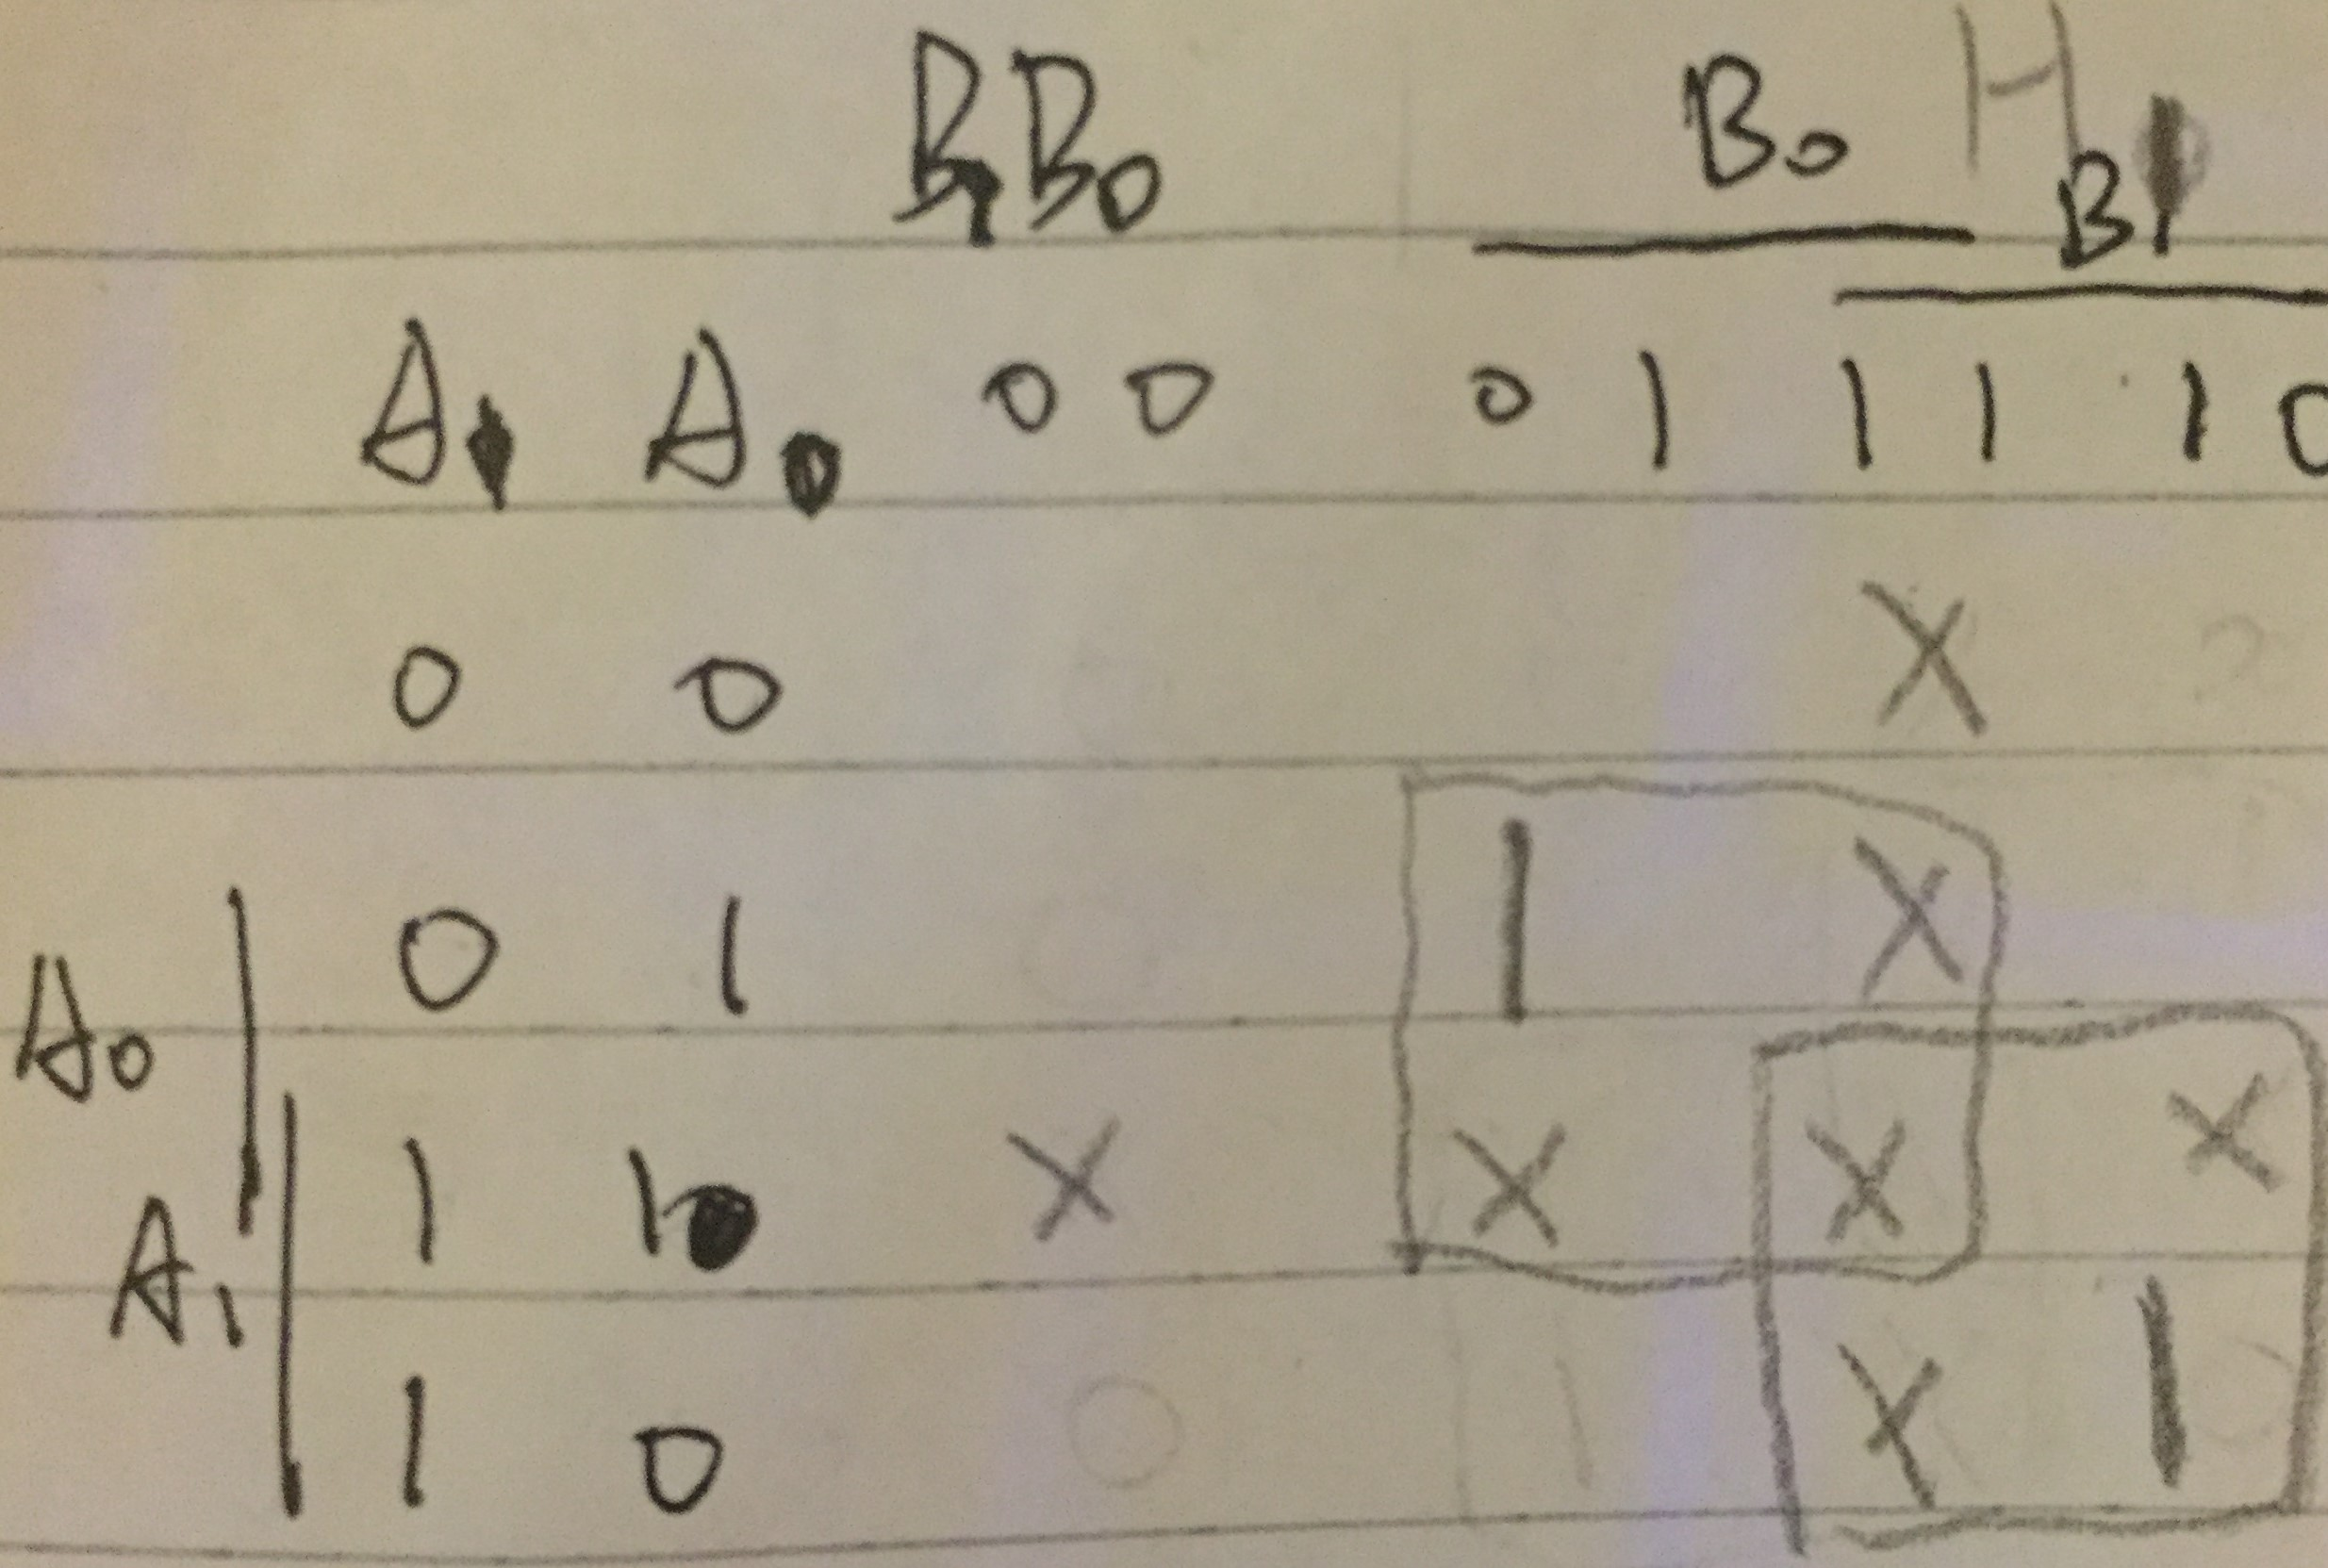
\includegraphics[scale=0.1]{7H0.JPG} 
$H_0 =A_0 B_0 + A_1 B_1$\newline
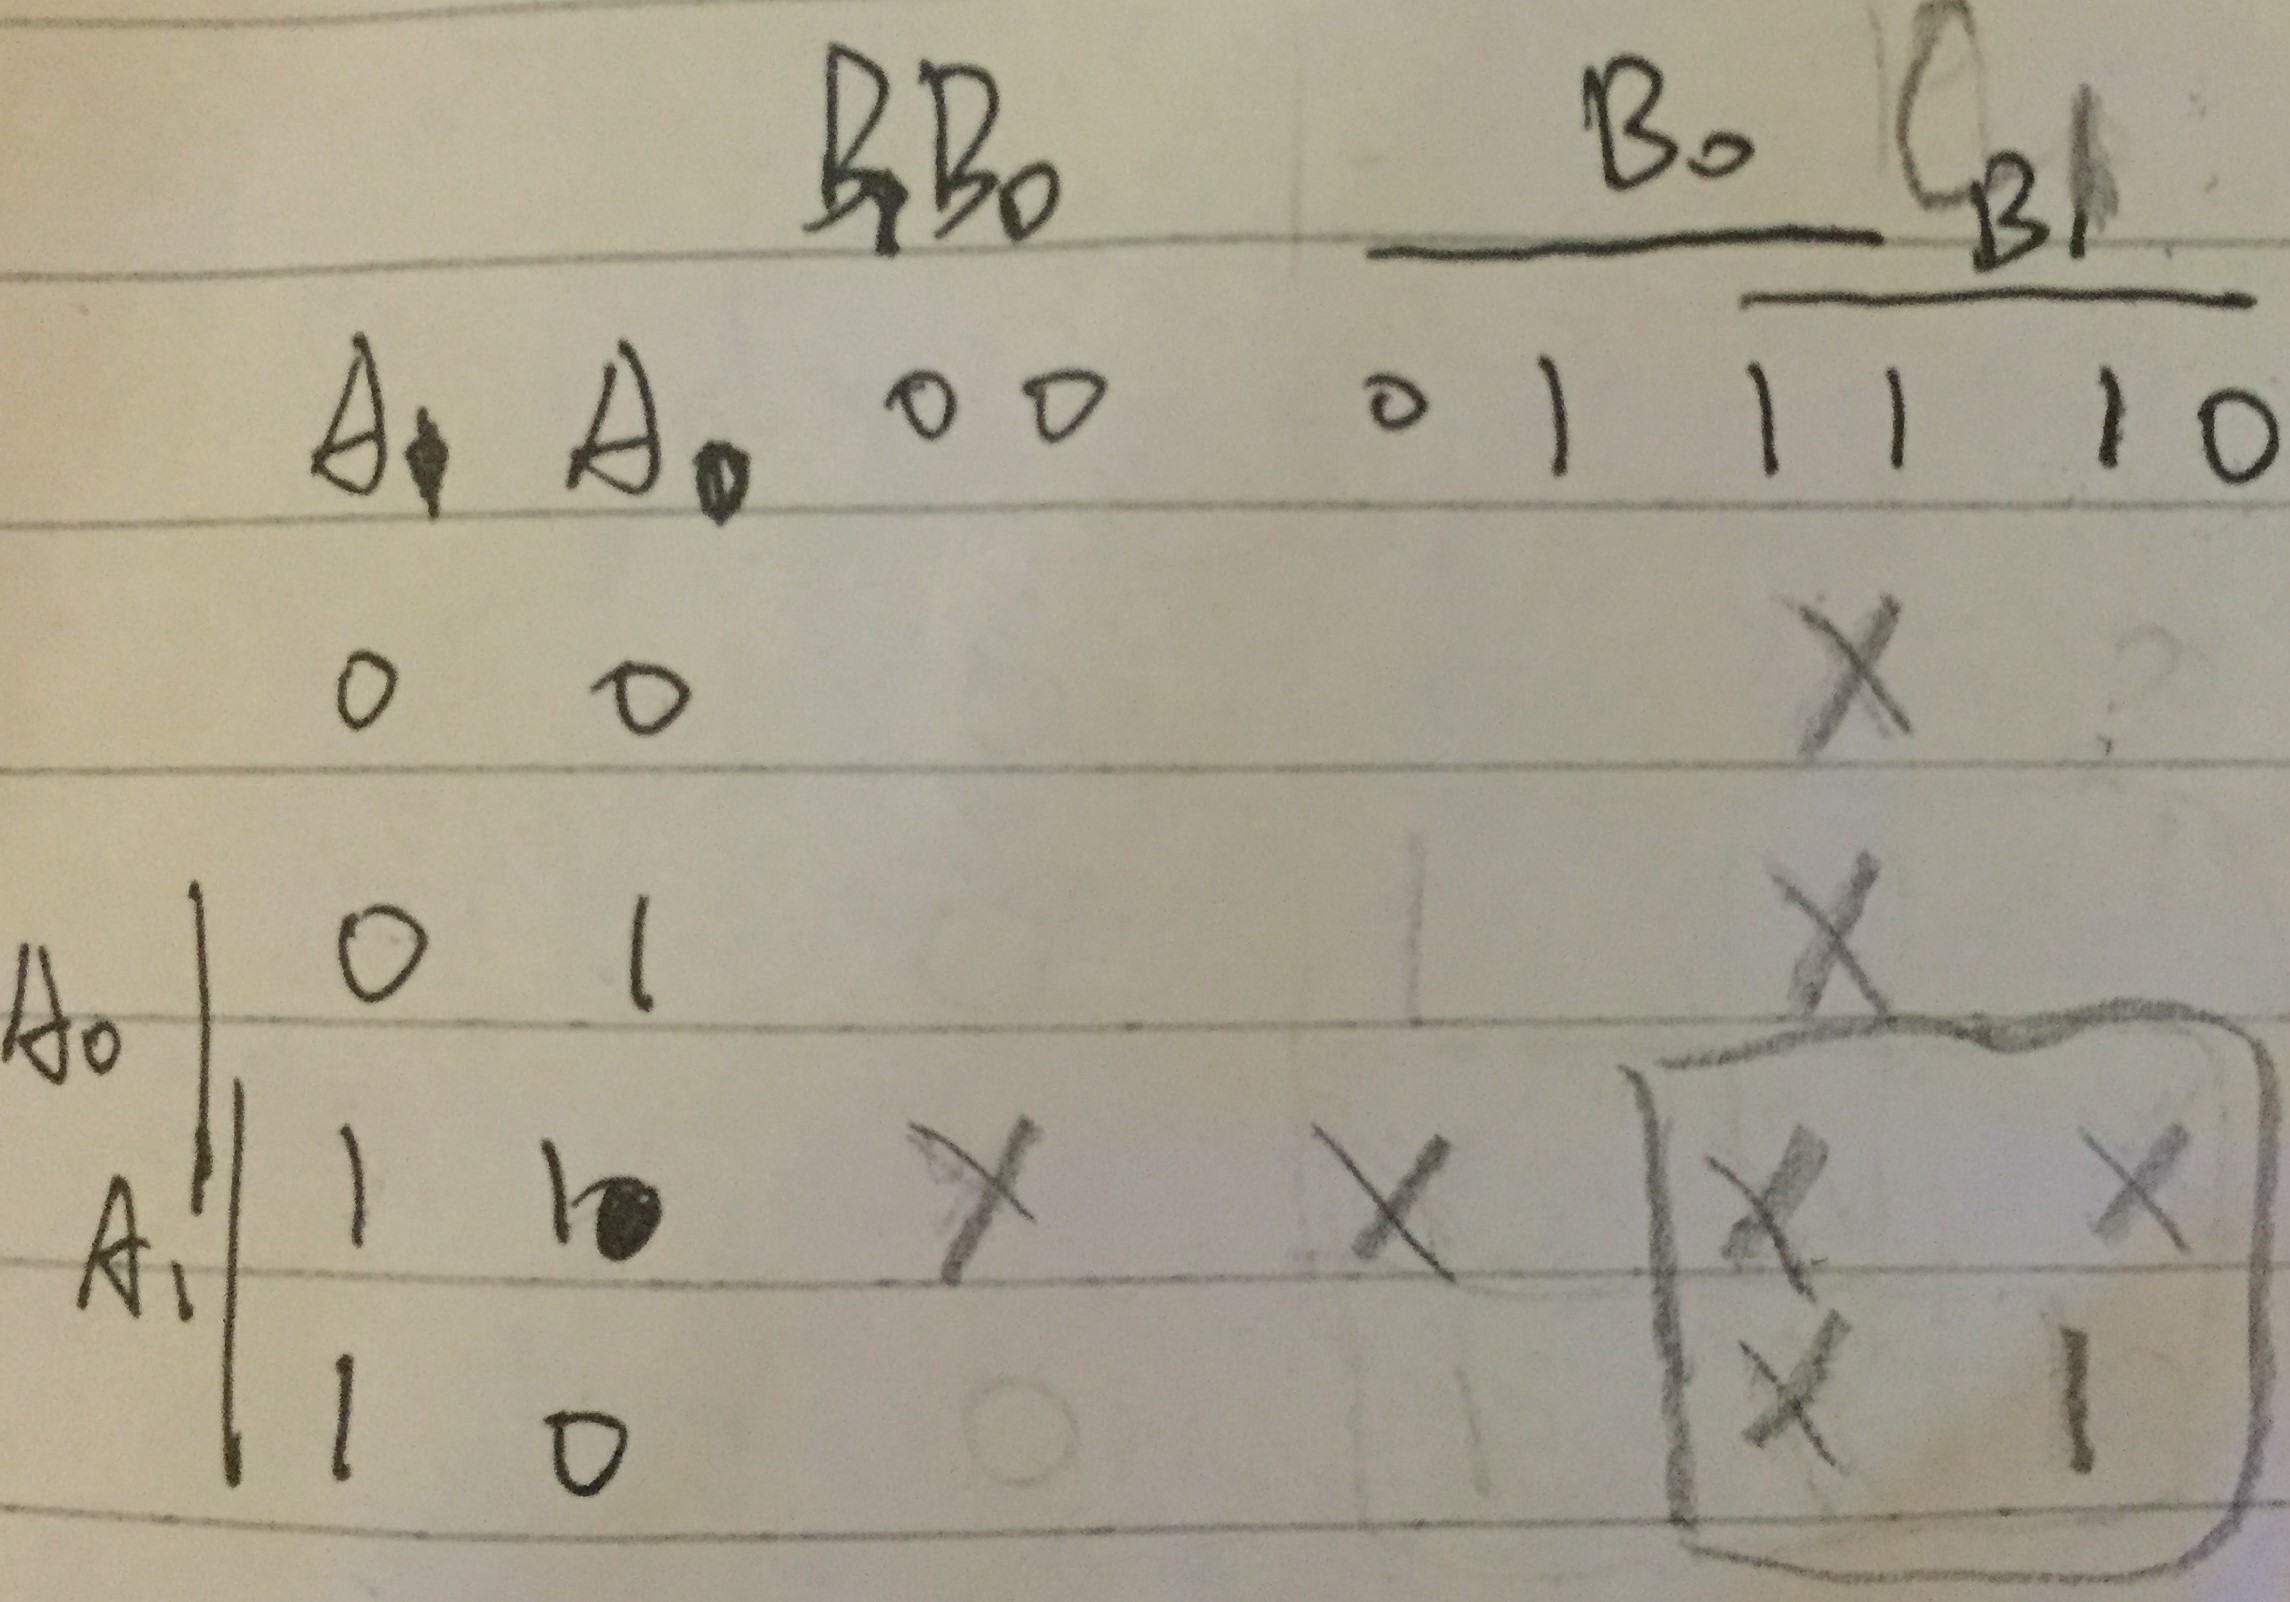
\includegraphics[scale=0.1]{7C1.JPG} 
$C_1 =A_1 B_1$\newline
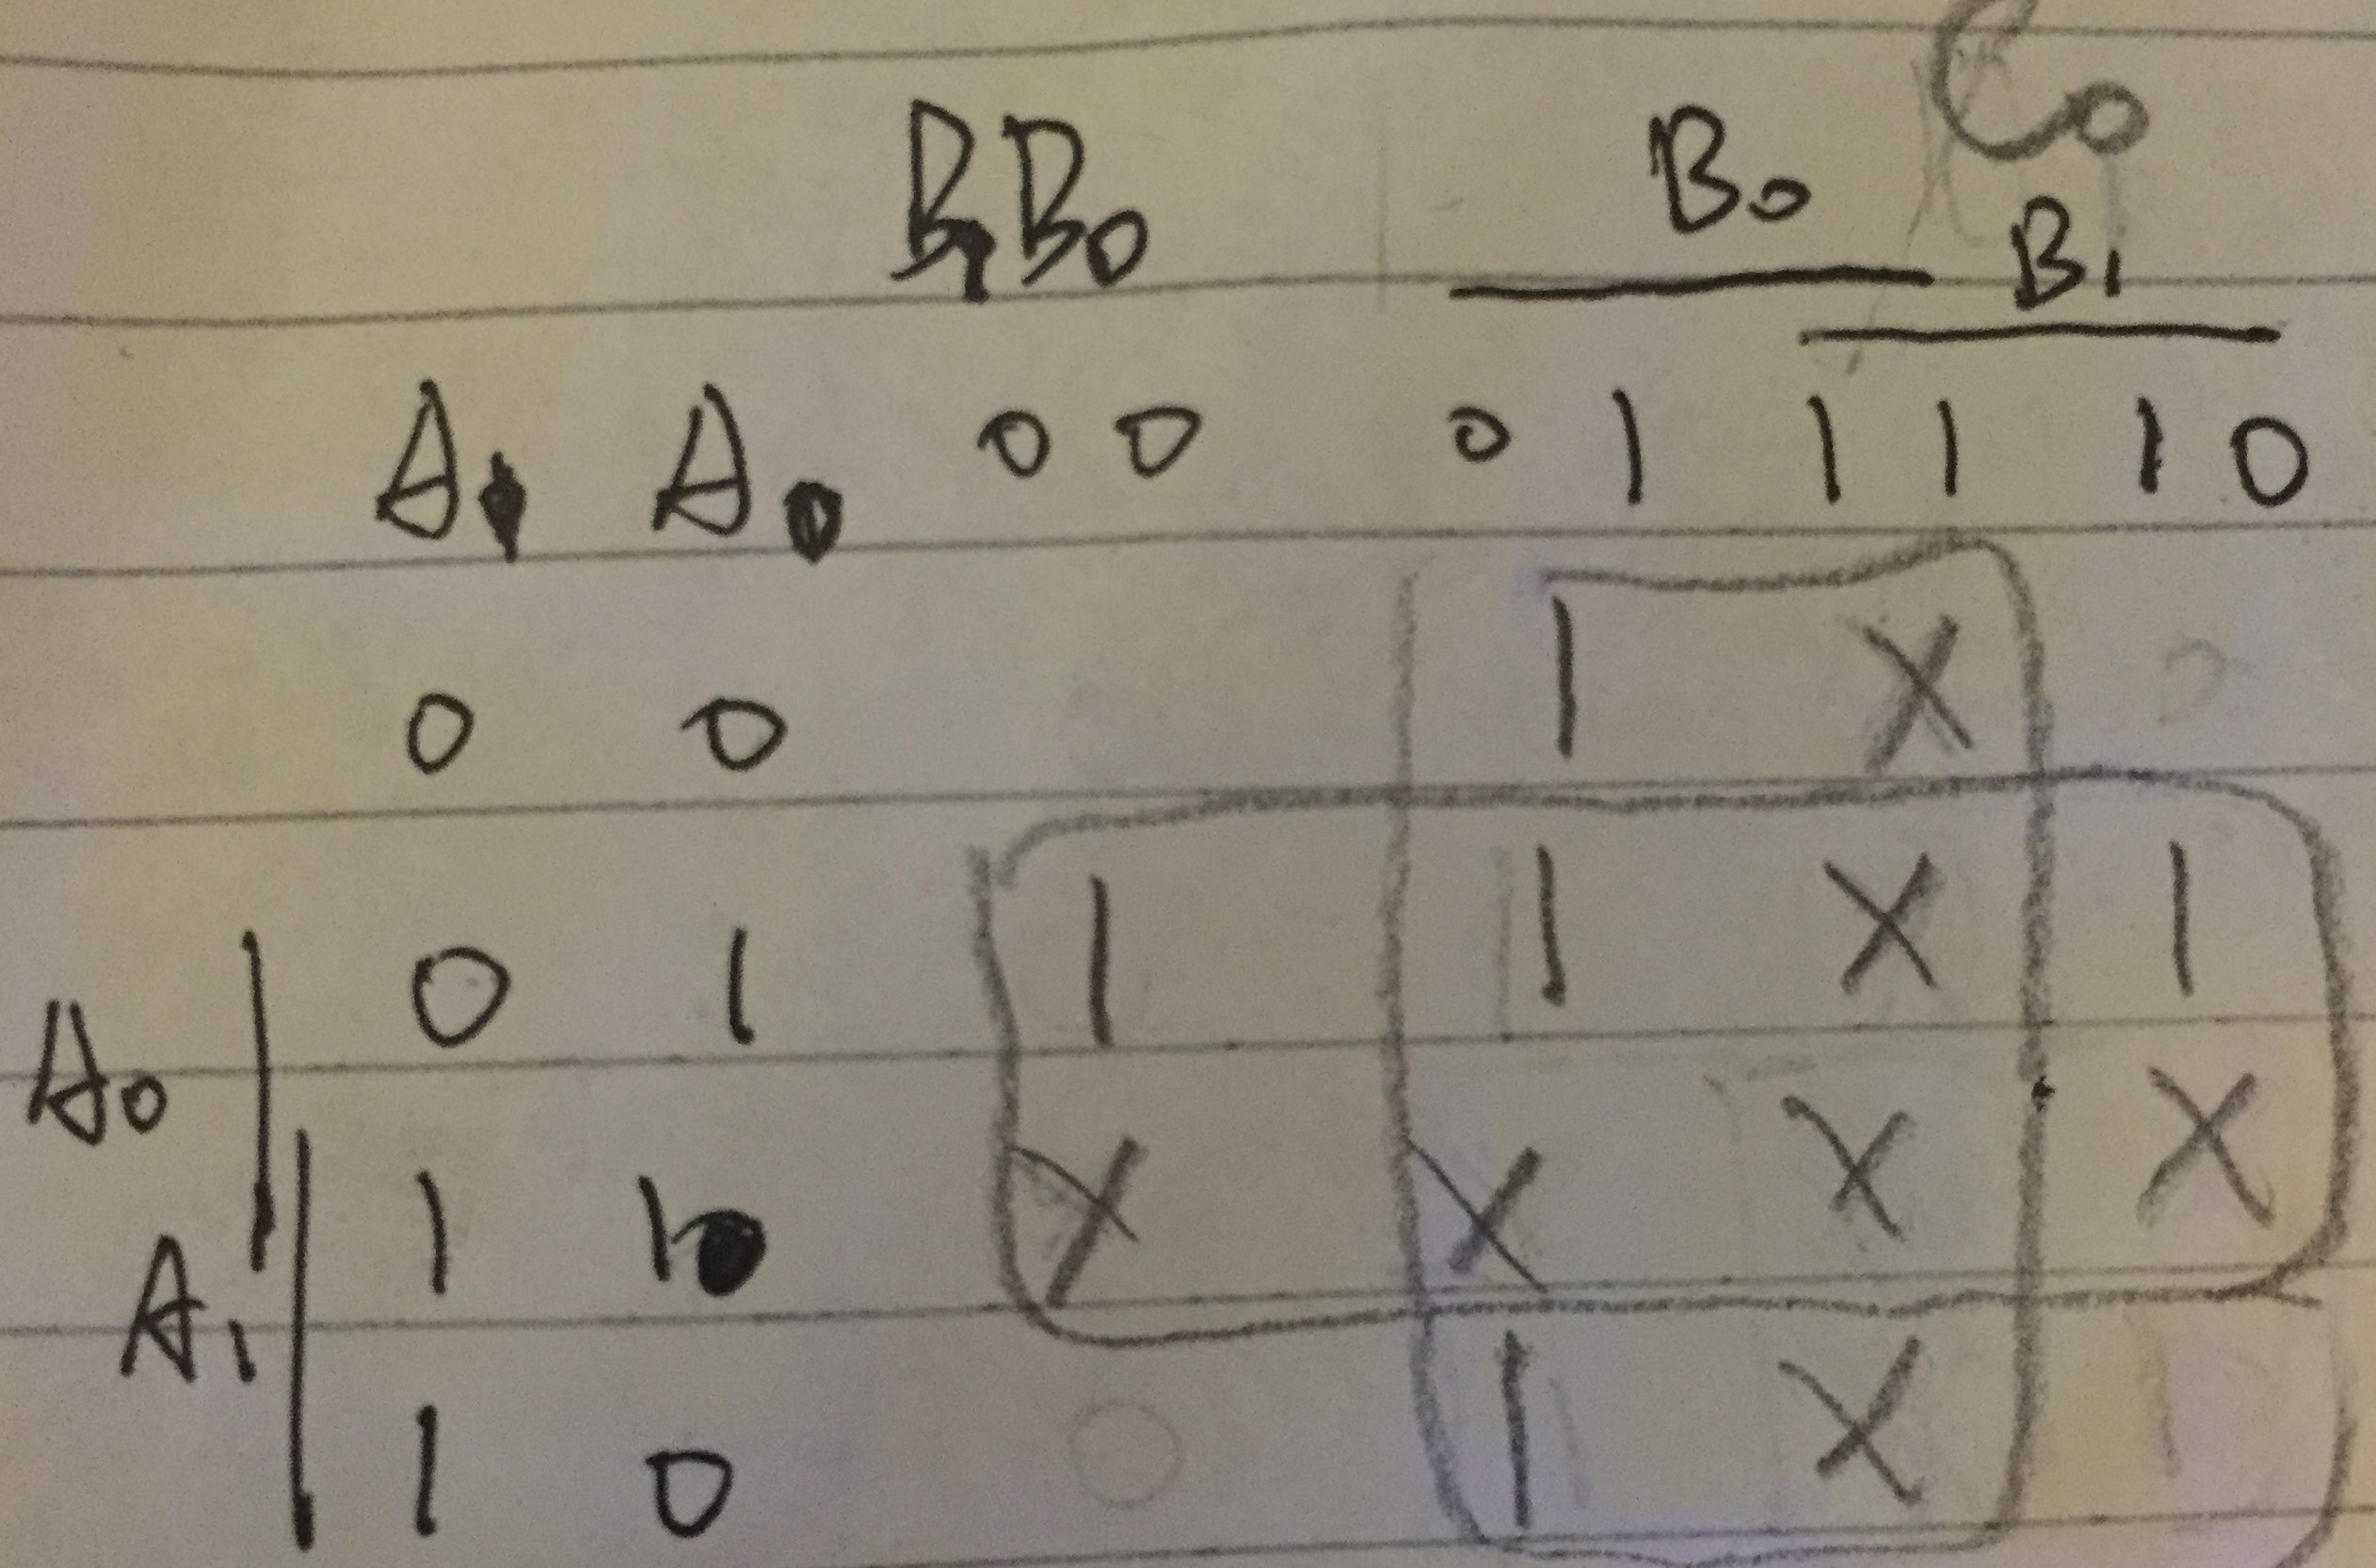
\includegraphics[scale=0.09]{7C0.JPG} 
$C_0 =A_0 + B_0$\newline

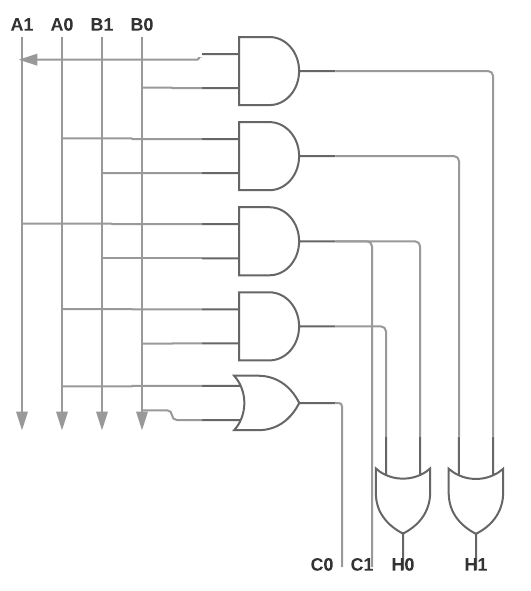
\includegraphics[scale=1]{7(1).png} 

\item[(c)]
This needs 7 gates. Original circuit needs 3 gates.

\item[(d)]
They both have $2T$ (ps) delay.

\end{enumerate}


\section{Ex8}

\begin{enumerate}
\item[(a)]
$\bar{U}=U\bar{X}+\bar{U}\bar{W}\bar{Y}+\bar{U}\bar{W}\bar{Z}+\bar{U}\bar{Z}Y+X\bar{W}\bar{U}$
\item[(b)]
This is exactly the same as Ex5(e).\newline
As change A to U, B to W, C to X, D to Y, E to X.\newline
so $P=UX+\bar{U}\bar{Y}W+\bar{U}WZ+\bar{U}\bar{X}YZ$

\item[(c)]
picture \newline

\includegraphics[scale=0.8]{8.png} 

\end{enumerate}




% End of your supervision work
%
%%%%%%%%%%%%%%%%%%%%%

\end{document}

